\documentclass[12pt]{article}
\usepackage[a4paper, total={7in,10in}]{geometry}

\usepackage{polyglossia}
\usepackage{ragged2e}
\usepackage{amsmath}
\usepackage{amssymb}
\usepackage{microtype}
\usepackage{graphicx}
\usepackage{changepage}
\usepackage{hyperref}
\usepackage{cancel}
\usepackage{wrapfig}
\usepackage{needspace}
\usepackage{mathtools}
\usepackage{tikz}
\usepackage{esint}
\newcommand*\circled[1]{\tikz[baseline=(char.base)]{
    \node[shape=circle, draw, inner sep=1pt, 
        minimum height=12pt] (char) {#1};}}



\let\ORIincludegraphics\includegraphics
\renewcommand{\includegraphics}[2][]{\ORIincludegraphics[scale=0.65,#1]{#2}}
\newcommand{\verteq}{\rotatebox{90}{$\,=$}}
\newcommand{\equalto}[2]{\underset{\scriptstyle\overset{\mkern4mu\verteq}{#2}}{#1}}
\let\oldint\int
\let\oldiint\iint
\let\oldiiint\iiint
\let\oldoint\oint
\let\oldsum\sum
\let\oldlim\lim
\let\oldoiint\oiint
\renewcommand{\int}{\oldint\limits}
\renewcommand{\oint}{\oldoint\limits}
\renewcommand{\iint}{\oldiint\limits}
\renewcommand{\oiint}{\oldoiint\limits}
\renewcommand{\iiint}{\oldiiint\limits}
\renewcommand{\sum}{\oldsum\limits}
\renewcommand{\lim}{\oldlim\limits}

\graphicspath{{./images/}}
\setmainlanguage{russian}
\setotherlanguage{english}
\newfontfamily\russianfont[Script=Cyrillic]{Times New Roman}
\newfontfamily\englishfont{Times New Roman}
\setlength{\parindent}{0em}
\setlength{\parskip}{6pt}

\def\posl#1#2{\{#1_{#2}\}}
\DeclareMathOperator*{\sh-like}{\sinh-like}
\DeclareMathOperator*{\ch-like}{\cosh-like}
\DeclareMathOperator*{\th-like}{\tanh-like}
\DeclareMathOperator*{\cth-like}{\coth-like}
\DeclareMathOperator*{\tg-like}{\tan-like}
\DeclareMathOperator*{\ctg-like}{\cot-like}
\DeclareMathOperator*{\arctg-like}{\arctan-like}
\DeclareMathOperator*{\arcctg-like}{\arctan-like}

\setcounter{section}{7}

\begin{document}
    \justifying
    \begin{titlepage}
        \begin{center}
            \begin{center}
              
\includegraphics[scale=0.1]{logo.jpg}
            \end{center}
            \normalsize{МИНИСТЕРСТВО НАУКИ И ВЫСШЕГО ОБРАЗОВАНИЯ РОССИЙСКОЙ ФЕДЕРАЦИИ}\\
            \footnotesize{ФЕДЕРАЛЬНОЕ ГОСУДАРСТВЕННОЕ АВТОНОМНОЕ ОБРАЗОВАТЕЛЬНОЕ УЧРЕЖДЕНИЕ}\\ 
            \footnotesize{ВЫСШЕГО ОБРАЗОВАНИЯ}\\
            \small{\textbf{«Дальневосточный федеральный университет»}}\\
            \noindent\rule{17cm}{0.4pt}\\
            \large{\textbf{ИНСТИТУТ МАТЕМАТИКИ И КОМПЬЮТЕРНЫХ ТЕХНОЛОГИЙ}}\\
             \hfill \break
            \large{\textbf{Департамент программной инженерии и искусственного интеллекта}}\\
            \hfill\break
            \hfill \break
            \hfill \break
            \hfill \break
            \large{\textbf{ЛЕКЦИОННЫЙ МАТЕРИАЛ}}\\
            \begin{center}
              \normalsize{по дисциплине "Математический Анализ"}\\
              \normalsize{по образовательной программе подготовки бакалавров по направлению}\\
              \normalsize{02.03.03тп - Математическое Обеспечение и Администрирование Информационных систем}\\
              \normalsize{семестры обучения III-IV}
            \end{center}
            \hfill \break
            \hfill \break
            \hfill \break
            \begin{flushright}
                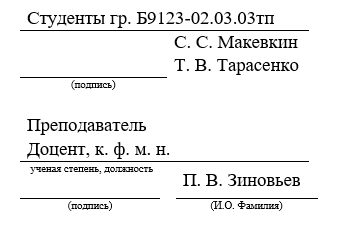
\includegraphics[scale=1.5]{rospis.png}
            \end{flushright}
            \hfill \break
            
            \end{center}
            \hfill \break
            \normalsize{ 
            
            }
            \begin{center} Владивосток \\ 2025 \end{center}
            \thispagestyle{empty}
    \end{titlepage}
    \pagebreak
    \tableofcontents
    \pagebreak
  \section{Криволинейные, кратные и поверхностные интегралы}
  \subsection{Криволинейные интегралы I рода}
  \underline{Определение: } Кривая $\overline{r}(t)=x(t)\overline{i}+y(t)\overline{j}+z(t)\overline{k} \hspace{10pt}$
  $a \leq t \leq b$ называется непрерывной гладкой кривой, если x(t),y(t),z(t) непрерывно дифференцируемы
  на [a;b] и $x'(t)^2+y'(t)^2+z'(t)^2 \not = 0$\\
  \underline{Определение: } Кривая называется непрерывной кусочно-гладкой кривой, если она состроит из конечного числа
  гладких кривых.\\
  Рассмотрим непрерывную кусочно-гладкую кривую:\\
  \begin{minipage}{0.45\textwidth} % Левая колонка — для изображения
      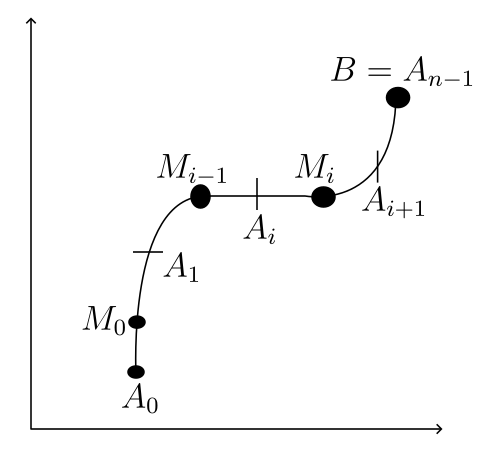
\includegraphics[width=\linewidth]{8.1.1.png}
  \end{minipage}%
  \hspace{1em} % Горизонтальный отступ между колонками
  \begin{minipage}{0.65\textwidth} % Правая колонка — для текста
      Пусть кривая имеет массу $\rho=\frac{\mathrm{kg}}{\mathrm{m}}$.
      \begin{enumerate}
        \item R
        \item В каждой элементарной $\Delta l_i$ выберем\\ произвольную $M_i$ 
        \item Вычислим $\rho(M_i)$
        \item Считаем, что на всём $\Delta l_i \rho=const=\rho(M_i)$
        \item Составим $\sigma_R=\sum_{i=0}^{n-1}\rho(M_i)\Delta l_i$
        \item $\lim_{\lambda_R \to 0} \sigma_R = m = \int_{(l)} g dl$
      \end{enumerate}
  \end{minipage}
  \vspace{1em}
  \par Рассмотрим функцию Z=f(x,y), заданную вдоль непрерывной кусочно-гладкой кривой l\\

  \begin{minipage}{0.45\textwidth}
    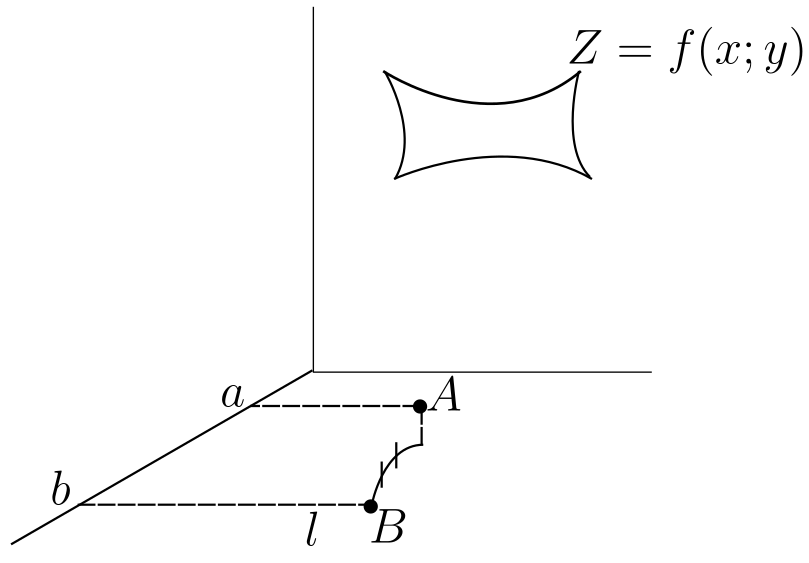
\includegraphics[scale=0.6]{8.1.2.png}
  \end{minipage}
  \hspace{1em} % Горизонтальный отступ между колонками
  \begin{minipage}{0.65\textwidth} % Правая колонка — для текста
      Пусть кривая имеет массу $\rho=\frac{\mathrm{kg}}{\mathrm{m}}$.
      \begin{enumerate}
        \item R
        \item Выберем произвольную (.) $M_i \in \Delta l_i$\\ (.)$M_i (\xi_i;\eta_i)$
        \item Вычислим $f(\xi_i;\eta_i)$
        \item Составим $\sigma_R = \sum_{i=0}^{n-1} f(\xi_i,\eta_i) \Delta l_i$
        \item Вычислим $\lim_{\lambda_R \to 0} \sigma_R = \int_{(l)} f(x;y) dl$
      \end{enumerate}
  \end{minipage}
  \vspace{1em}
  \par
  \underline{Определение: } Если существует конечный предел интегральной суммы $\sigma_R$, не 
  зависящей от способа разбиения кривой и выбора $(.) M_i(\xi_i,\eta_i)$, то он называется
  криволинейным интегралом I рода от функции f(x;y) по кривой l.\\
  \[m=\int_{(l)} f(x;y) dl\]\\
  \underline{Замечание:} Если кривая (AB) не замкнута: \[\int_{(AB)} f(x;y)dl = \int_{(BA)} f(x;y)dl\]
  !!! При переходе к определенному интегралу пределы интегрирования ставятся по мере возрастания
  переменной интегрирования.

  \begin{minipage}{0.45\textwidth}
    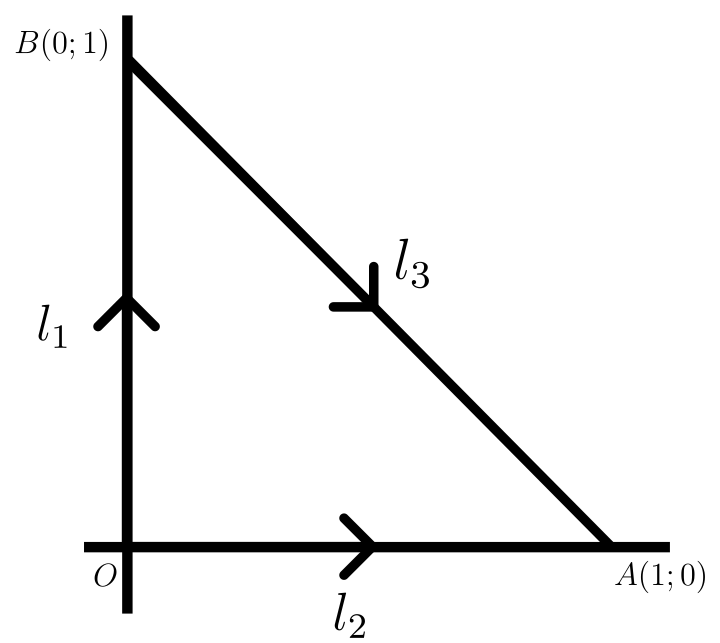
\includegraphics[scale=0.6]{8.1.3.png}
  \end{minipage}
  \hspace{1em}
  \begin{minipage}{0.65\textwidth}
      \[\int = \int_{(l_1)}+\int_{(l_2)}+\int_{(l_3)}\]\\
      \[\int_{0}^{1}\dots dy+\int_{0}^{1}\dots dx+\int_{0}^{1}\dots dx\]
  \end{minipage}
  \vspace{1em}
  \par
  \underline{Замечание:} Аналогично вводится интеграл по пространственной кривой $\int_{(l)} f(x;y;z)dl$
  \subsection{Вычисление криволинейного интеграла I рода.}
  \[\int_{(l)} f(x;y) dl \hspace{10pt} l: \begin{cases}
    x=x(t) & a\leq t\leq b\\
    y=y(t)
  \end{cases}\] \\
  \begin{minipage}{0.45\textwidth}
    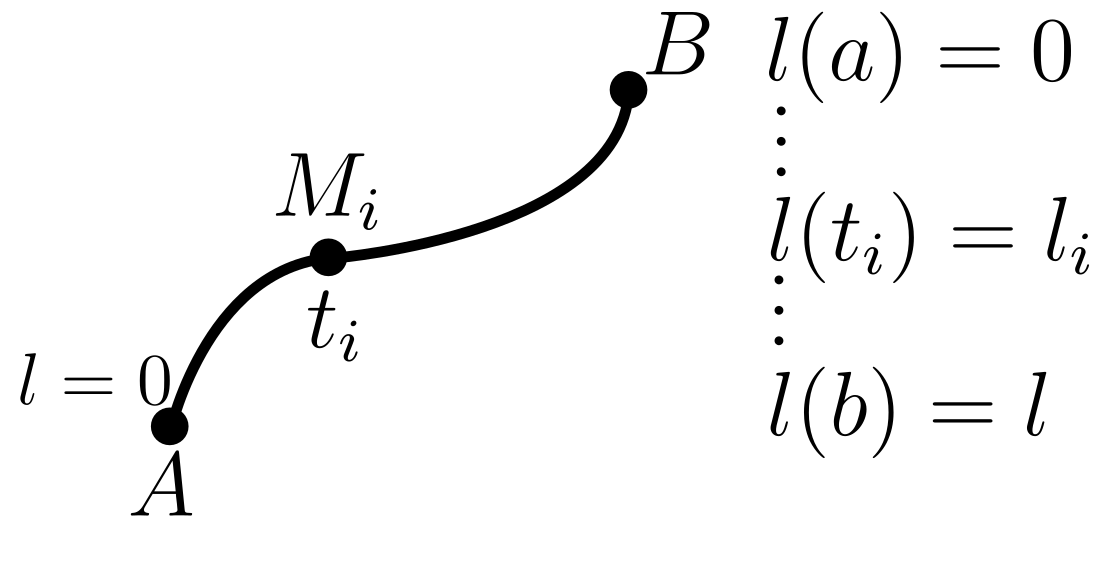
\includegraphics[scale=0.4]{8.2.1.png}
  \end{minipage}
  \hspace{1em}
  \begin{minipage}{0.65\textwidth}
    Положение (.) $M_i$ однозначно определяется с помощью \\
    длины дуги, отсчитываемой от (.)A. $\begin{cases}
      x=x(l)\\
      y=y(l)
    \end{cases}$
  \end{minipage}
  \vspace{1em}
  \par
  \[\int_{(l)}f(x;y)dl=\int_{0}^{l} f(x(l);y(l))dl\]
  \begin{enumerate}
    \item Если кривая задана уравнением y=f(x) $a \leq x \leq b$\\
    \[\int_{(l)} g(x;y)dl = \int_{a}^{b} f(x) \underbrace{\sqrt{1+f'(x)^2}dx}_{dl}\]
    \item Если кривая задана параметрически\\
    \[\begin{cases}
      x=x(t)\\
      y=y(t)
    \end{cases} t_1 \leq t \leq t_2 \hspace{20pt} \int_{(l)}g(x;y)dl=\int_{t_1}^{t_2}g(x(t);y(t))
    \sqrt{x'(t)^2+y'(t)^2}dt\]
    \item Если кривая задана $r=r(\varphi) \hspace{20pt} \alpha \leq \varphi \leq \beta$\\
    \[\int_{(l)}g(x;y)dl = \int_{\alpha}^{\beta} g(r(\varphi)\cos(\varphi);r(\varphi)\sin(\varphi))
    \sqrt{r^2(\varphi)+r'(\varphi)^2}d\varphi\]
  \end{enumerate}
  \subsection*{Свойства криволинейных интегралов I-рода:}
  \begin{enumerate}
    \item $\int_{(l)}dl=L$
    \item m=$\int_{(l)}\rho dl$
    \item $x_c=\frac{M_y}{m}=\frac{\int_{(l)}\rho xdl}{\int_{(l)}\rho dl}$ \hspace{20pt}
    $M_y$ - статический момент кривой относительность оси y.\\
    $y_c = \frac{M_x}{m}=\frac{\int_{(l)}\rho ydl}{\int_{(l)}\rho dl}$ \hspace{20pt}
    $M_x$ - статический момент кривой относительно оси X
  \end{enumerate}
  \subsection{Криволинейные интегралы II рода}
  Пусть задана Z=f(x;y), которая определена в каждой (.) l\\
  \begin{minipage}{0.45\textwidth}
    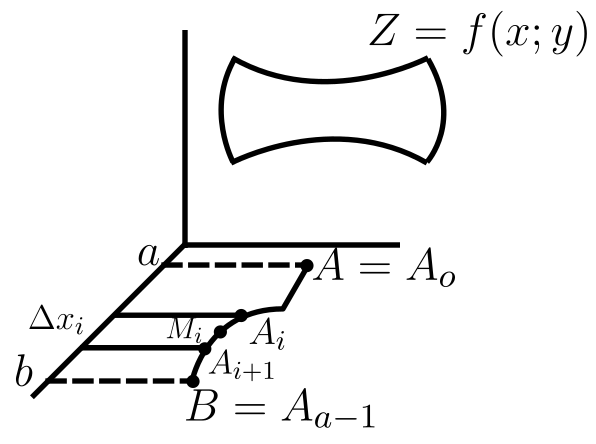
\includegraphics[scale=0.8]{8.3.1.png}
  \end{minipage}
  \hspace{1em}
  \begin{minipage}{0.65\textwidth}
    \begin{enumerate}
      \item R
      \item $M_i(\xi_i,\eta_i) \in \Delta l_i$
      \item $f(M_i)=f(\xi_i;\eta_i)$
      \item $\sum_{i=0}^{n-1}f(\xi_i;\eta_i)\Delta x_i=\sigma_R$
      \item $\lim_{\lambda_R \to 0}\sigma_R=\int_{(l)}f(x;y)dx$
    \end{enumerate}
  \end{minipage}
  \vspace{1em}
  \par
  \underline{Определение: } Если существует конечный предел суммы $\sigma_R$, не зависящей от способа
  разбиения кривой l и выбора (.) $M_i(\xi_i;\eta_i)$, то он называется криволинейным интегралом
  II рода от функции f(x;y) по кривой l\\
  \underline{Замечание:} Аналогично вводится\\
  \[\int_{(l)}f(x;y)dy\]\\
  Если вдоль кривой определенны функции $P(x;y),Q(x;y)$ и существует $\int_{(AB)}P(x;y)dx$ и
  $\int_{(AB)}Q(x;y)dy$, то $\int_{(AB)}P(x;y)dx+Q(x;y)dy$ называется криволинейным интегралом
  II рода общего вида.\\
  \underline{Замечание:} \[\int_{(AB)}f(x;y)dx=-\int_{(BA)}f(x;y)dx\]\\
  Аналогично вводится: \[\int_{(AB)}P(x;y;z)dx+Q(x;y;z)dy+R(x;y;z)dz\]
  \subsection{Существование и вычисление криволинейного интеграла II рода}
  \subsubsection*{Теорема 8.4.1}\label{th:8.4.1}
  \par\noindent
  Пусть кривая AB задана параметрически:\\
  $\begin{cases}
    x=\varphi(t) \hspace{20pt} \varphi(t),\psi(t) \text{ непрерывны } \forall t \in [a;b]\\
    y=\psi(t)
  \end{cases}$\\
  Пусть f=f(x;y) непрерывна вдоль кривой AB. $\varphi'(t)$ существует и непрерывна $\forall t \in [a;b]$.
  Тогда существует криволинейный интеграл $\int_{(AB)}f(x;y)dx=\int_{a}^{b}f(\varphi(t);\psi(t))\varphi'(t)dt$\\
  \underline{Доказательство:}
  \begin{adjustwidth}{1.5em}{1.5em}
    \begin{minipage}{0.45\textwidth}
      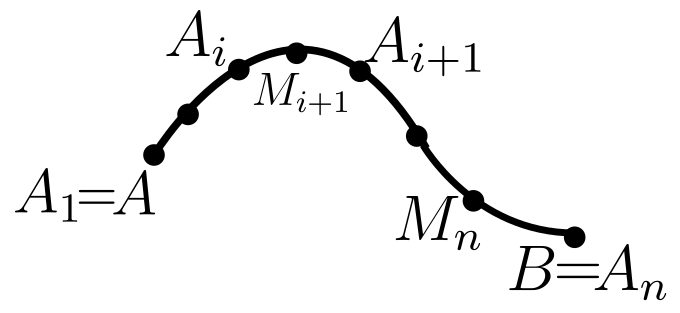
\includegraphics[scale=0.6]{8.4.1.png}
    \end{minipage}
    \hspace{1em}
    \begin{minipage}{0.55\textwidth}
      \begin{enumerate}
        \item Произведем разбиение R кривой (AB) точками $A_i(\varphi(t_i);\psi(t_i))$
        \item Выберем (.) $M_i(\varphi(\tau_i);\psi(\tau_i))$
        \item $\Delta x_i = \varphi(t_{i+1})-\varphi(t_i)=\int_{t_i}^{t_{i+1}}\varphi'(t)dt$
        \item $\sigma_R=\sum_{i=0}^{n-1}f(\varphi(\tau_i);\psi(\tau_i))\Delta x_i=\\=\sum_{i=0}^{n-1}
        f(\varphi(\tau_i);\psi(\tau_i))\int_{t_i}^{t_{i+1}}\varphi'(t)dt$
      \end{enumerate}
    \end{minipage}
    \vspace{1em}
    \par
  \end{adjustwidth}
  Рассмотрим правую часть: $\int f(\varphi(\tau_i);\psi(\tau_i))\varphi'(t)dt = \sum_{i=1}^{n}
    \int_{t_i}^{t_{i+1}}f(\varphi(\tau_i);\psi(\tau_i))\varphi'(t)dt=I$\\
  Рассмотрим $|\sigma_R-I|=\sum_{i=1}^{n} \int_{t_i}^{t_{i+1}} [f(\varphi(\tau_i);\psi(\tau_i))-
  f(\varphi(t);\psi(t))]\varphi'(t)dt \boxed{<}$\\
  Т.к. f(x;y) непрерывна вдоль кривой (AB)\\
  \[\forall \varepsilon >0 \exists \delta = \delta(\varepsilon):|\Delta t_i| < \delta \Rightarrow
  |f(\varphi(t_{i+1});\psi(t_{i+1}))-f(\varphi(t_i);\psi(t_i))|<\varepsilon\]\\
  или $\begin{matrix}
    [t_i;\tau_i] <[t_i;t_{i+1}]\\
    [\tau_i;t_{i+1}] < [t_i;t_{i+1}]
  \end{matrix} \hspace{20pt} \varphi'(t)$ непрерывна на $[t_i;t_{i+1}] \Rightarrow$ она ограничена на нём.\\
  Пусть $\forall i |\varphi'(t_i)|<L$\\
  \boxed{<} $|\varepsilon L \sum_{i=1}^{n} \int_{t_i}^{t_{i+1}}dt|=\varepsilon L(b-a)\Rightarrow \lim_{\lambda_R \to 0}\sigma_R=I$
  \begin{center}
    \textbf{Ч.т.д.}
  \end{center}
  Аналогично: \[\int_{(AB)}f(x;y)dy=\int_{a}^{b}f(\varphi(t);\psi(t))\psi'(t)dt\]\\
  Если кривая задана как y=y(x) \hspace{10pt} $a\leq x\leq b$. Тогда\\
  $\begin{cases}
    y=y(t)\\
    x=t
  \end{cases} \hspace{20pt} a\leq t\leq b \Rightarrow \int_{(AB)}f(x;y)dx =\int_{a}^{b} f(t;y(t))dt=
  |x=t|=\int_{a}^{b}f(x;y(x))dx$\\
  \underline{Замечание:} $\int_{(AB)}f(x;y)dx=0,$ если AB-прямоугольный отрезок || оси OY. Аналогично \\
  $\int_{(CD)}f(x;y)dy=0,$ если CD-прямоугольный отрезок || OX.\\
  Если L-замкнутый контур.\\
  \begin{minipage}{0.45\textwidth}
    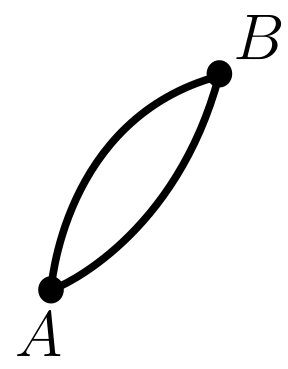
\includegraphics[scale=0.6]{8.4.2.png}
  \end{minipage}
  \hspace{1em}
  \begin{minipage}{0.25\textwidth}
    \[\int_{(l)}=\int_{(AB)}+\int_{(BA)}\]
  \end{minipage}
  \vspace{1em}
  \par
  Среди двух возможных обходов, L обход против часовой стрелки, причём за положительный обход. При обходе рассматриваемая область
  находится слева.
  \subsection{Вычисление площади криволинейной трапеции с помощью криволинейного интеграла.}
  \begin{minipage}{0.45\textwidth}
    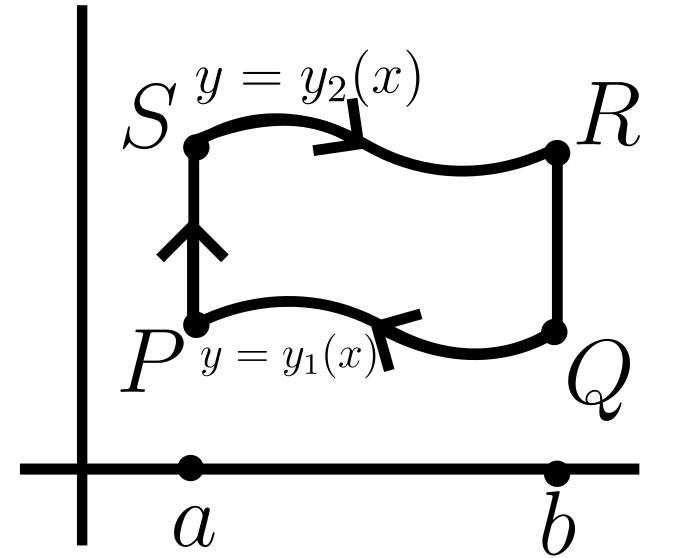
\includegraphics[scale=0.6]{8.5.1.png}
  \end{minipage}
  \hspace{1em}
  \begin{minipage}{0.55\textwidth}
    \begin{center}
      Найти S(PSRQ)
    \end{center}
    \[S=\int_{a}^{b}y_2(x)dx-\int_{a}^{b}y_1(x)dx \boxed{=}\]
     \[\text{Рассмотрим} \int_{a}^{b}y_2(x)dx=\int_{(SR)}ydx\]
      \[\text{Рассмотрим}\int_{a}^{b}y_1(x)dx=\int_{(PQ)}ydx\]
  \end{minipage}
  \vspace{1em}
  \[\boxed{=} \int_{(SR)}ydx-\int_{(PQ)}ydx=\int_{(SR)}ydx+\int_{(QP)}ydx+\int_{(PS)}ydx+\int_{(RQ)}ydx=\int_{(PSRQP)}ydx \boxed{=}\]
  \par
  Пусть L=(PQRSP) - контур взятый в положительном направлении. $\boxed{=}-\int_{(L)}ydx=S$\\
  Аналогично, если рассмотреть:
  \begin{flushleft}
    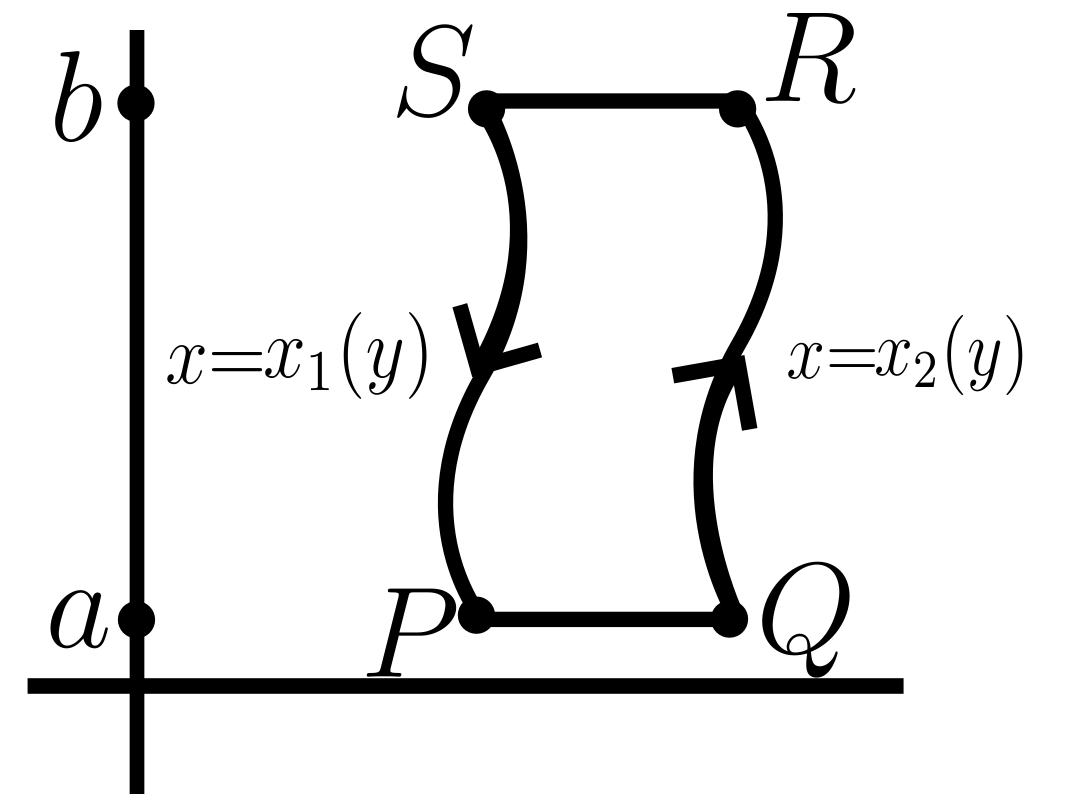
\includegraphics[scale=0.4]{8.5.2.png}
  \end{flushleft}
  То получим S=$\int_{(l)}xdy$\\
  Для произвольного замкнутого контура L\\
  \[\boxed{S=\frac{1}{2}\int_{(l)}xdy-ydx}\]
  \underline{Замечание:}
  \begin{flushleft}
      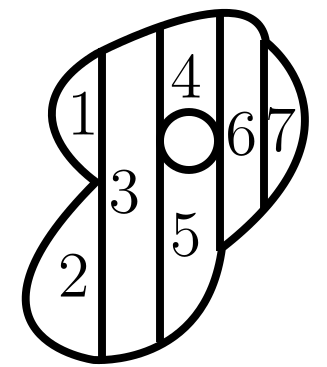
\includegraphics{8.5.3.png}
  \end{flushleft}
  \subsection{Связь между криволинейными интегралами I и II рода}
  Пусть кривая задана в виде $\overline{r}=\overline{r}(t) \hspace{20pt} a\leq t \leq b$\\
  \begin{flushright}
    $\overline{r}=\overline{r}(x(t^*);y(t^*))$
  \end{flushright}
  \begin{figure}[h!]
    \centering
    % Первая колонка (левая картинка)
    \begin{minipage}{0.45\textwidth}
        \centering
        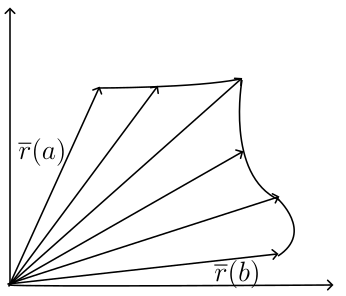
\includegraphics[width=\textwidth]{8.6.1.png} % путь к первой картинке
        \vspace{0.5em} % небольшой отступ между картинкой и текстом
        $\Delta \overline{r}=\overline{r}(t_o+\Delta t)-\overline{r}(t_0)$\\
        $\frac{\Delta \overline{r}}{\Delta t}=\frac{1}{\Delta t}*\Delta \overline{r}$\\
        $\lim_{\Delta t \to 0} \frac{\Delta \overline{r}}{\Delta t}=r(t_0)$\\
        $|\overline{r}'(t)|=l'(t)$
    \end{minipage}
    \hfill
    % Вторая колонка (правая картинка)
    \begin{minipage}{0.45\textwidth}
        \centering
        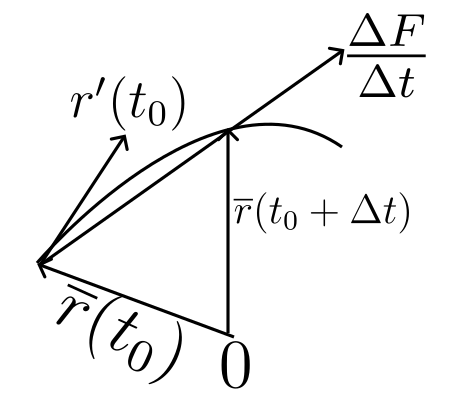
\includegraphics[width=\textwidth]{8.6.2.png} % путь ко второй картинке
        \vspace{0.5em} % небольшой отступ между картинкой и текстом
        $\overline{r}'(t)=\overline{x'(t);y'(t)}$\\
        $|\overline{r}'(t)=\sqrt{x'(t)^2+y'(t)^2}|$\\
        $dl=\sqrt{x'(t)^2+y'(t)^2}dt|:dt$\\
        $l'(t)=\sqrt{x'(t)^2+y'(t)^2}$
    \end{minipage}
  \end{figure}
  \par
  Пусть l-переменная длина дуги\\
  \[\frac{d \overline{r}}{dl} = \frac{d \overline{r}}{dt}* \frac{dt}{dl}=\frac{\frac{d \overline{r}}{dt}}{\frac{dl}{dt}}
  \hspace{20pt} \Big| \frac{d \overline{r}}{dt} \Big| = \Big| \frac{r'(t)}{l'(t)} \Big| = 1\]\\
  \underline{Замечание:} Если $|\overline{a}|=1 \Rightarrow \overline{a}(\cos(\alpha),\cos(\beta),\cos(\gamma))
  \hspace{20pt} \cos^2 \alpha+\cos^2 \beta+\cos^2 \gamma=1$\\
  \[\frac{d \overline{r}}{dl}=(\overline{\cos \alpha; \cos \beta})=(\overline{\frac{dx}{dl};\frac{dy}{dl}})\]
  \[\frac{dx}{dl}=\cos \alpha \hspace{20pt} dx=\cos \alpha dl\]
  \[\frac{dy}{dl}=\cos \beta \hspace{20pt} dy=\cos \beta dl\]
  Рассмотрим $\int_{(l)}f(x;y)dx=\int_{(l)}f(x;y)\cos \alpha dl$\\
  В общем случае $\int_{(l)}P(x;y;z)dx+Q(x;y;z)dy+R(x;y;z)dz=$\\
  \[\int_{(l)} [P(x;y;z)\cos \alpha + Q(x;y;z)\cos \beta + R(x;y;z)\cos \gamma]dl\]
  \subsection*{Физический смысл криволинейным интеграла II рода}
  Рассмотрим $\int_{(l)} Pdx+Qdy+Rdz$\\
  Пусть F(P;Q;R) - сила, под действием которой (.) перемещается по кривой l.\\
  d $\overline{S}(dx;dy;dz)$\\
  Рассмотрим $\overline{F}*\overline{ds}=A$\\
  Криволинейный интеграл II рода равен работе силы F по перемещению (.) по кривой l.
  \subsection{Условие независимости криволинейного интеграла от путей интегрирования.}
  Рассмотрим $\begin{matrix}
    P=P(x;y)\\
    Q=Q(x;y)
  \end{matrix}$\\
  Рассмотрим $\int_{(AB)}Pdx+Qdy \boxed{1}$\\
  Найти условия, при которых значение интеграла не зависит от вида кривой (AB) и однозначно определяется положением
  (.) A и (.) B\\
  Рассмотрим Pdx+Qdy \hspace{20pt} dF = $\frac{\delta F}{\delta x}dx + \frac{\delta F}{\delta y}dy$\\
  Если $P=\frac{\delta F}{\delta x} \hspace{20pt} Q=\frac{\delta F}{\delta y}$, то Pdx+Qdy является полными
  дифференциалом от некоторой F(x;y).\\
  \subsubsection*{Теорема 8.7.1}\label{th:8.7.1}
  \par\noindent
  $\Leftrightarrow$ чтобы Pdx+Qdy было в рассматриваемой области дифференциалом от некоторой функции 
  F(x;y)\\
  \underline{Доказательство:}
  \begin{adjustwidth}{1.5em}{1.5em}
    $\Rightarrow$ пусть \boxed{1} не зависит от путей интегрирования \\
    \hspace{1em}
    \begin{minipage}{0.55\textwidth}
      \[\int_{(AB)} Pdx+Qdy = \int_{(x_0;y_0)}^{(x_1;y_1)}Pdx+Qdy\]\\
      \[\text{Рассмотрим F(x;y)=}\int_{(x_0;y_0)}^{(x;y)}Pdx+Qdy\]
    \end{minipage}
    \vspace{1em}
    \begin{minipage}{0.45\textwidth}
      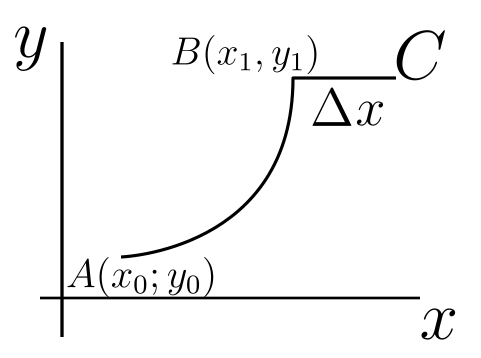
\includegraphics[scale=0.6]{8.7.1.png}
    \end{minipage}
    \par
    \[F(x;y)=\int_{(x_0;y_0)}^{(x_1;y_1)}Pdx+Qdy\]\\
    \[F(x_1+\Delta x;y_1)=\int_{(x_0;y_0)}^{(x_1+\Delta x;y_1)}Pdx+Qdy=\int_{(AB)}Pdx+qdy+
    \int_{(CD)}Pdx+Qdy\]\\
    Рассмотрим $F(x_1+\Delta x,y_1)-F(x_1;y_1)=\int_{(BC)}Pdx=\int_{x_1}^{x_1+\Delta x}P(x;y_1)dx=
    \Big| \text{\underline{Замечание:}} \int_{a}^{b}f(x)dx=f(\xi)(b-a)\Big| = \underset{\xi \in (x_1;x_1+\Delta x)}{P(\xi;y_1)}
    \Delta x = \underset{0<\theta<1}{P(x_1+\theta \Delta x;y_1)}\Delta x$\\
    \[\frac{F(x_1+\Delta x;y_1)-F(x_1;y_1)}{\Delta x} = P(x_1+\theta\Delta x;y_1)\]\\
    \[\lim_{\Delta x \to 0} \frac{F(x_1+\Delta x;y_1)-F(x_1;y_1)}{\Delta x}=\frac{\delta F}{\delta x} \Big|_{(x_1;y_1)}
    =P(x;y)\Big|_{(x_1;y_1)}\]\\
    \[\forall x \in D \hspace{20pt} \frac{\delta F}{\delta x}=P(x;y)\]\\
    Аналогично $\frac{\delta F}{\delta y}=Q(x;y)$\\
    $\Leftarrow$ Пусть Pdx+Qdy=$\frac{\delta F}{\delta x}+\frac{\delta F}{\delta y}dy$\\
    \[\int_{(l)}Pdx+Qdy= \begin{vmatrix}
      x=\varphi(t) & \varphi(a)=x_a & \varphi(b)=x_b\\
      y=\psi(t) & \psi(a)=y_a & \psi(b)=y_b  \\
      dx=\varphi'(t)dt\\
      dy=\psi'(t)dt
    \end{vmatrix} = \int_{a}^{b}[P(\varphi(t);\psi(t))\varphi'(t)+Q(\varphi(t);\psi(t))\psi'(t)]dt=\]\\
    \[=\int_{a}^{b}[\frac{\delta F}{\delta x}\varphi'(t)+\frac{\delta F}{\delta y}\psi'(t)]dt=\int_{a}^{b}
    \frac{dF(\varphi(t);\psi(t))}{dt}dt=F(\varphi(t);\psi(t))\Big|^b_a= F(x_b;y_b)-F(x_a;y_a)\]
    \begin{center}
      \textbf{Ч.т.д.}
    \end{center}
  \end{adjustwidth}
  \begin{center}
    Как установить, является ли выражение Pdx+Qdy полным дифференциалом?\\
    $Pdx+Qdy \overset{?}{=} dF$\\
    Если $\begin{matrix}
      P=\frac{\delta F}{\delta x} & Q=\frac{\delta F}{\delta y}\\
      \frac{\delta P}{\delta y}=\frac{\delta^2 F}{\delta y \delta x} & \frac{\delta Q}{\delta x}=\frac{\delta^2 F}{\delta x \delta y}
    \end{matrix} \Rightarrow \frac{\delta P}{\delta y}= \frac{\delta Q}{\delta x}$
  \end{center}
  
  
  \begin{minipage}{0.55\textwidth}
    \underline{Вопрос}: Как найти функцию F(x;y)?\\
    \[\int_{(l)}dF=F(x;y)+C\]\\
    Зафиксируем (.)$(x_0;y_0)$
  \end{minipage}
  \hspace{1em}
  \begin{minipage}{0.45\textwidth}
    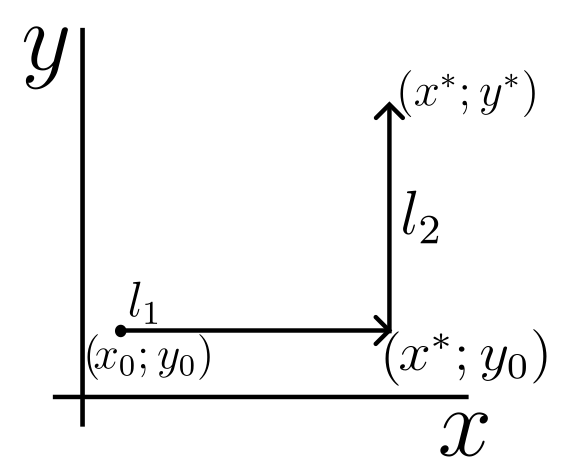
\includegraphics[scale=0.6]{8.7.2.png}
  \end{minipage}
  \vspace{1em}
  \par
  $\begin{matrix}
    \text{(x,y) - произвольная (.) области } & \hspace{20pt} & l_1: y=y_0 & dy=0\\
    \text{Обозначим её} (x^*;y^*) & \hspace{20pt} & l_2:x=x^x & dx=0
  \end{matrix}$\\
  \[\int_{(l)}Pdx+Qdy=\int_{(l_1)}Pdx+Qdy+\int_{(l_2)}Pdx+Qdy+C = \int_{x_0}^{x^*}P(x;y_0)dx+
  \int_{y_0}^{y^x}Q(x^*;y)dy+C=F(x^*;y^*)\]
  \subsection{Интеграл по замкнутому контуру}
  Рассмотрим $\int_{(l)}Pdx+Qdy$ L-замкнутый контур в положительном направлении.
  \begin{center}
    \underline{Вопрос:} При каких условиях интеграл по замкнутому контуру обращается в ноль?
  \end{center}
  \subsubsection*{Теорема 8.8.1}\label{th:8.8.1}
  \par\noindent
  Если $\int_{(AB)}Pdx+Qdy$ не зависит от пути интегрирования, то $\int_{(l)}Pdx+Qdy=0.$Верно и обратное утверждение.\\
  \begin{minipage}{0.25\textwidth}
    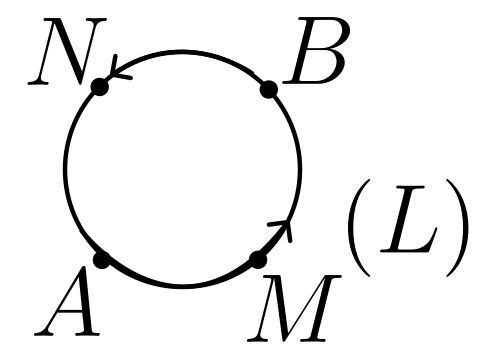
\includegraphics[scale=0.5]{8.8.1.png}
  \end{minipage}
  \hspace{1em}
  \begin{minipage}{0.75\textwidth}
    \underline{Доказательство:}\\
      $\Rightarrow : \int_{(AB)}Pdx+Qdy$ не зависит от пути интегрирования.\\
      $\int_{(AMB)}=\int_{(AMB)} \Rightarrow \int_{(AMB)}-\int_{(AMB)}=0 \Rightarrow
      \Rightarrow \int_{(AMB)}+\int_{(BNA)}=0 \Rightarrow \int_{(L)}=0$
  \end{minipage}
  \vspace{1em}
  \par
  $\Leftarrow:$ Пусть $\int_{(L)}=0$
  \begin{center}
    $\int_{(AMB)}+\int_{(BNA)}=0$\\
    $\int_{(AMB)}=-\int_{(BNA)}$\\
    $\int_{(AMB)}=\int_{(ANB)}$\\
  \end{center}
  \begin{center}
    \textbf{Ч.т.д.}
  \end{center}
  \underline{Замечание:} Существует область, для которых условие $\frac{\delta P}{\delta y}=\frac{\delta Q}{\delta x}$
  не является достаточным для того, чтобы криволинейный интеграл не зависел от пути интегрирования.\\
  \par
  \underline{Определение: } Область, для которой $\forall$ расположенный в ней замкнутый контур можно путём
  непрерывной деформации стянуть в (.), не выходя за пределы области, называется односвязной. В противном
  случаем - неодносвязной.\\
  \par
  \begin{minipage}{0.5\textwidth}
    односвязный\\
    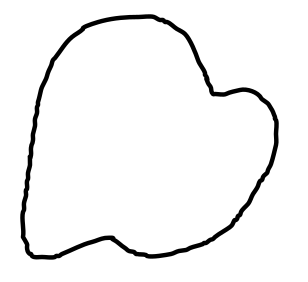
\includegraphics[scale=0.6]{8.8.2.png}
  \end{minipage}
  \hspace{1em}
  \begin{minipage}{0.5\textwidth}
      не односвязный\\
    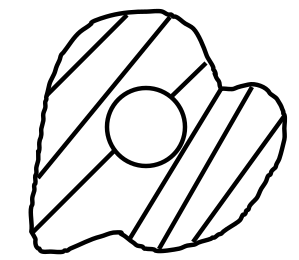
\includegraphics[scale=0.6]{8.8.3.png}
  \end{minipage}
  \vspace{1em}
  \par
  \textbf{Утверждение:} Для того, чтобы\\
  \[\oint_{(L)} Pdx+Qdy=0 \text{ необходимо, а в случае односвязной области достаточно, чтобы } \frac{\delta P}{\delta y}=\frac{\delta Q}{\delta x}\]
  Рассмотрим контур, имеющий внутри себя особую точку\\
  \textbf{Утверждение:} Пусть $\frac{\delta P}{\delta y}=\frac{\delta Q}{\delta x}$. Тогда
  \begin{enumerate}
    \item $\oint_{L}Pdx+Qdy$ может быть отличным от нуля.
    \item Все интегралы взятые в "+" направлении, по $\forall$ замкнутому контуру, будут равны между собой.
  \end{enumerate}
  \underline{Доказательство:}\\
  2)
  \begin{minipage}{0.45\textwidth}
    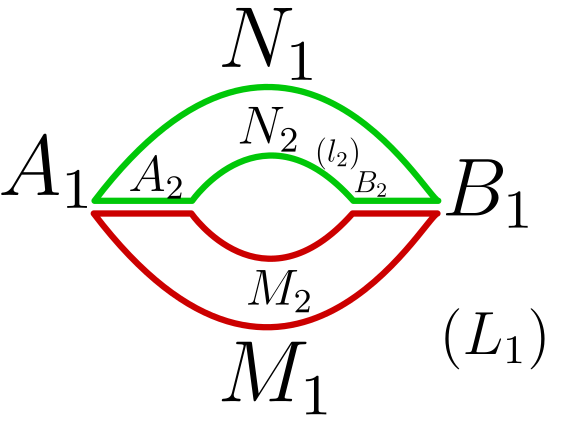
\includegraphics[scale=0.6]{8.8.4.png}
  \end{minipage}
  \hspace{1em}
  \begin{minipage}{0.55\textwidth}
    Рассмотрим \\
    \[\begin{matrix}
      \int_{(A_1M_1B_1)}+\int_{B_1B_2}+\int_{B_2M_2A_2}+\int_{A_1A_1} = 0\\
      \int_{B_1N_1A_1}+\int_{A_1A_2}+\int_{A_2N_2B_2}+\int_{B_2B_1} =0 
    \end{matrix} \Bigg\} \Rightarrow\] 
    \[\Rightarrow \int_{A_1M_1B_1N_1A_1} + \int_{B_2M_2N_2N_2B_2} =0 \]
    \[\int_{A_1M_1B_1N_1A_1}=-\int_{B_2M_2A_2N_2B_2}\]
    \[\int_{(l_1)}=\int_{(l_2)}\]
  \end{minipage}
  \vspace{1em}
  \begin{center}
    \textbf{Ч.т.д.}
  \end{center}
  Рассмотрим $\oint_{(L)} Pdx+Qdy=\sigma$\\
  \begin{minipage}{0.45\textwidth}
    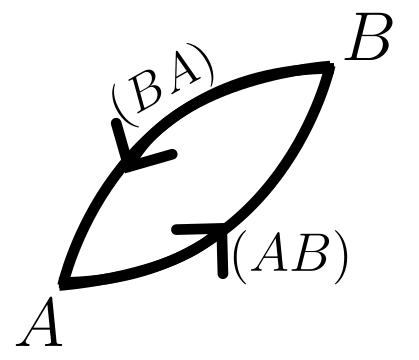
\includegraphics[scale=0.6]{8.8.5.png}
  \end{minipage}
  \hspace{1em}
  \begin{minipage}{0.4\textwidth}
    \[\int_{(AB)}Pdx+Qdy+\int_{(BA)}Pdx+Qdy=n\sigma\]
    \[\int_{(AB)}Pdx+Qdy=\int_{(AB)}Pdx+Qdy+n\sigma\]
  \end{minipage}
  \vspace{1em}
  \par
  То есть интеграл зависит от пути интегрирования. В смысле прибавления кратного числа к циклической
  постоянной.\\
  Присоединив к кривой AB некоторое число петель, окружающих особую (.), можно добиться, чтобы криволинейный
  интеграл принял значение, близкое к заданному.\\
  \underline{Пример:} $\oint_{(L)} \frac{xdy-ydx}{x^2+y^2} \boxed{=} \hspace{20pt} L:x^2+y^2=a^2, r=a$\\
  \begin{minipage}{0.2\textwidth}
    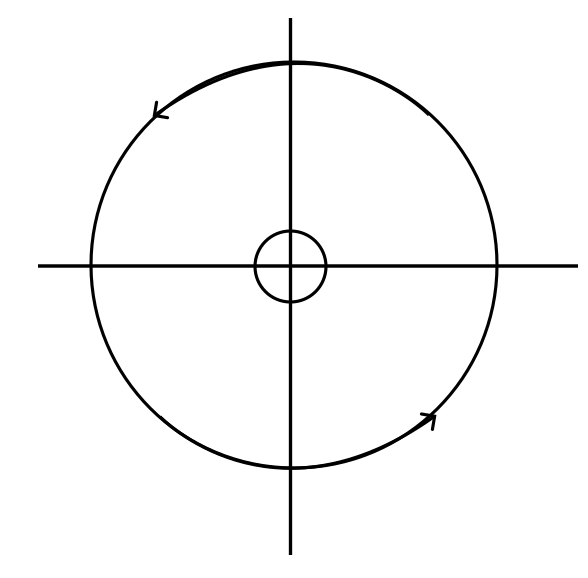
\includegraphics[scale=0.4]{8.8.6.png}
  \end{minipage}
  \hspace{1em}
  \begin{minipage}{0.8\textwidth}
    $P=\frac{-y}{x^2+y^2} \hspace{20pt} Q=\frac{x}{x^2+y^2} \hspace{10pt}$
    $\begin{matrix}
      x=r(\varphi)\cos(\varphi)=a\cos(\varphi) & dx=-a\sin(\varphi)d\varphi\\
      y=a\sin(\varphi) & dy=a\cos(\varphi)d\varphi
    \end{matrix}$
  \end{minipage}
  \vspace{1em}
  \par
  \[\boxed{=} \int_{0}^{2\pi} \frac{a^2\cos^2(\varphi)+a^2\sin^2(\varphi)}{a^2}d\varphi = 
  \int_{0}^{2\pi}d\varphi=\varphi \Big|^{2\pi}_0 = 2\pi = \sigma\]
  \begin{center}
    В общем случае $\oint_{(L)} Pdx+Qdy=n_1\sigma_1+n_2\sigma_2+\dots+n_k\sigma_k$
  \end{center}
  \subsection{Трёхмерный случай}
  Рассмотрим $\int_{(AB)}Pdx+Qdy+Rdz$\\
  Он не зависит от пути интегрирования, если существует F(x;y;z):
  \[\frac{\delta F}{\delta x}=P;\frac{\delta F}{\delta y}=Q;\frac{\delta F}{\delta Z}=R\]

  \[\text{Пусть существует непрерывные производные } \frac{\delta P}{\delta y};
  \frac{\delta P}{\delta z};\frac{\delta Q}{\delta x};\frac{\delta Q}{\delta z}
  ;\frac{\delta R}{\delta x};\frac{\delta R}{\delta y}\]

  \[\frac{\delta P}{\delta y}=\frac{\delta^2 F}{\delta y \delta x};
  \frac{\delta P}{\delta z}=\frac{\delta^2 F}{\delta z \delta x};
  \frac{\delta Q}{\delta x}=\frac{\delta^2 F}{\delta x \delta y};
  \frac{\delta Q}{\delta z}=\frac{\delta^2 F}{\delta z \delta y};
  \frac{\delta R}{\delta x}=\frac{\delta^2 F}{\delta x \delta z};
  \frac{\delta R}{\delta y}=\frac{\delta^2 F}{\delta y \delta z}\]

  \[\begin{matrix}
    \frac{\delta P}{\delta y} = \frac{\delta Q}{\delta x}\\
    \par \\
    \frac{\delta P}{\delta z} = \frac{\delta R}{\delta x}\\
    \par \\
    \frac{\delta Q}{\delta z} = \frac{\delta R}{\delta y}
  \end{matrix} \Bigg\} \text{- условие независимости криволинейного интеграла от пути интегрирования}\] 
  $P=\frac{\delta F}{\delta x}$\\
  Рассмотрим $\int_{x_0}^{x} P(x;y;z)dx=\int_{x_0}^{x}\frac{\delta F}{\delta x}dx = F(x;y;z)-F(x_0;y;z)$\\
  Зафиксируем $x_0. \int_{y_0}^{y}Q(x_0;y;z)dy=\int_{y_0}^{y}\frac{\delta F}{\delta y|_{x=x_0}}
  dy=F(x_0;y;z)-F(x_0;y_0;z)$\\
  Зафиксируем $x_0,y_0. \int_{z_0}^{z}R(x;y;z)dz=\int_{z_0}^{z}\frac{\delta F}{\delta z |_{x_0,y_0}}dz=
  F(x_0;y_0;z)-F(x_0;y_0;z_0)$
  \[F(x;y;z)=\int_{x_0}^{x}P(x;y;z)dx+\int_{y_0}^{y}Q(x_0;y;z)dy+\int_{z_0}^{z}R(x_0;y_0;z)dz+\equalto{F(x_0;y_0;z_0)}{C}\]
  \subsection{Кратные интегралы. Двойной интеграл в прямоугольной области.}
  \begin{minipage}{0.25\textwidth}
    Рассмотрим P: $\begin{matrix}
      a\leq x \leq b\\
      c \leq y \leq d
    \end{matrix}$
  \end{minipage}
  \hspace{1em}
  \begin{minipage}{0.45\textwidth}
    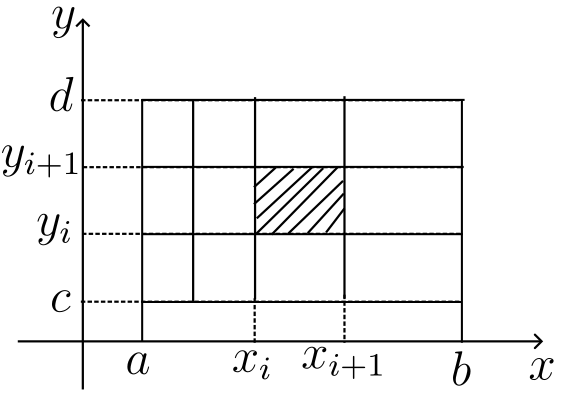
\includegraphics[scale=0.6]{8.10.1.png}
  \end{minipage}
  \vspace{1em}
  \par
  \begin{enumerate}
    \item R: $\begin{matrix}
      a=x_0 < x_1 < \dots < x_n =b\\
      c=y_0 <y_1 < \dots < y_n =d
    \end{matrix}$
    \item Выберем в каждом элементарном $P_{ij}$ произвольную (.) $(\xi_i;\eta_i)$
    \item Рассмотрим Z=f(x;y). Вычислим $f(\xi_i;\eta_i)$
    \item Вычислим $f(\xi_i;\eta_i)S_{P_{ij}}$
    \item Вычислим $\sum_{i=0}^{n-1} \sum_{j=0}^{m-1} f (\xi_i;\eta_i)S_{P_{ij}}$
    \item Обозначим $\lambda_R = max(d_{ij})$
    \item $\lim_{\lambda_R \to 0}\sigma_R=\iint_P f(x;y)dxdy$
  \end{enumerate}
  \underline{Определение: } Если существует конечный $\lim_{\lambda_R \to 0} \sigma_R$, не зависящий
  от способа разбиения R и выбора (.) $(\xi_i;\eta_i)$, то он называется двойным интегралом от f(x;y)
  по прямоугольнику P.\\
  \par\noindent
  \underline{Определение: } I называется двойным интегралом от f(x;y) по P, если 
  \[\forall \varepsilon > 0 \exists \delta =\delta(\varepsilon): \lambda_r < \delta \Rightarrow |I-\sigma_R| < \varepsilon\]

  \subsection{Суммы Дарбу}
  \[\overline{S}=\sum_{i=0}^{n-1} \sum_{j=0}^{m-1} M_{ij}\Delta x_i \Delta y_i = \sum_{i=1}^{n-1} \sum_{j=0}^{n-1}M_{ij}\Delta P_{ij}\]
  \[\underline{S}=\sum_{i=0}^{n-1} \sum_{j=0}^{m-1} m_{ij}\Delta x_i \Delta y_i = \sum_{i=1}^{n-1} \sum_{j=0}^{n-1}m_{ij}\Delta P_{ij}\]
  \[m_{ij} \leq f(x;y) \leq M_{ij} \hspace{20pt} \forall(x;y)\in P_{ij}\]
  \[M_{ij}=\underset{(x;y) \in \Delta P_{ij}}{sup f(x;y)} \hspace{20pt} m_{ij}=\underset{(x;y) \in \Delta P_{ij}}{inf f(x;y)} \]
  \subsection*{Свойства}
  \begin{enumerate}
    \item $\underline{S}\leq \sigma_R \leq \overline{S}, \forall R$
    \item Пусть $R \sqsubset R'$\\
    $\overline{S_{R'}}\leq \overline{S_{R}} \hspace{20pt} \underline{S_{R'}}\geq \underline{S_{R}}$
    \item $\forall R_1,R_2 \hspace{20pt} \underline{S_{R_1}}\leq \overline{S_{R_2}}$
    \item Множество верхних сумм Дарбу ограничено снизу.\par
    Множество нижних сумм Дарбу ограниченно сверху.\\
    $I_*=\underset{R}{sup \{\underline{S}\}} \hspace{20pt} I^*=\underset{R}{inf \{\underline{S}\}}$
    \item Th. о существовании интеграла\\
    f(x;y) интегрируема на P $\Leftrightarrow \lim_{\lambda_R \to 0} (\overline{S_R}-\underline{S_R})=0$\\
    $I_*=I^*=I$
  \end{enumerate}

  \subsection{Двойной интеграл в произвольной области}
  Пусть $\underset{\text{(квадратируема по Жордану)}}{\text{область D имеет конечную площадь}}$\\
  \begin{minipage}{0.45\textwidth}
    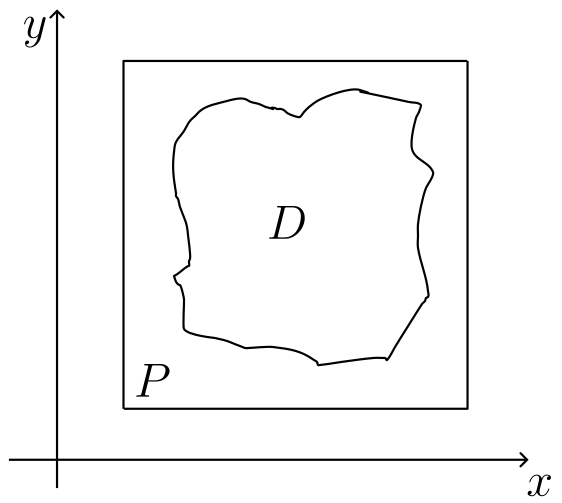
\includegraphics[scale=0.7]{8.12.1.png}
  \end{minipage}
  \hspace{1em}
  \begin{minipage}{0.55\textwidth}
    Пусть F(x;y)=$\begin{cases}
      f(x;y) & (.)(x;y) \in D\\
      0 & (.)(x;y) \not \in D
    \end{cases}$\\
    Если F(x;y) интегрируема в Р, то существует: \[\iint_{P} F(x;y)dxdy \]
    \[\iint_{P} F(x;y dxdy=\iint_{D} f(x;y)dxdy)\]
  \end{minipage}
  \vspace{1em}
  \par
  \begin{minipage}{0.45\textwidth}
    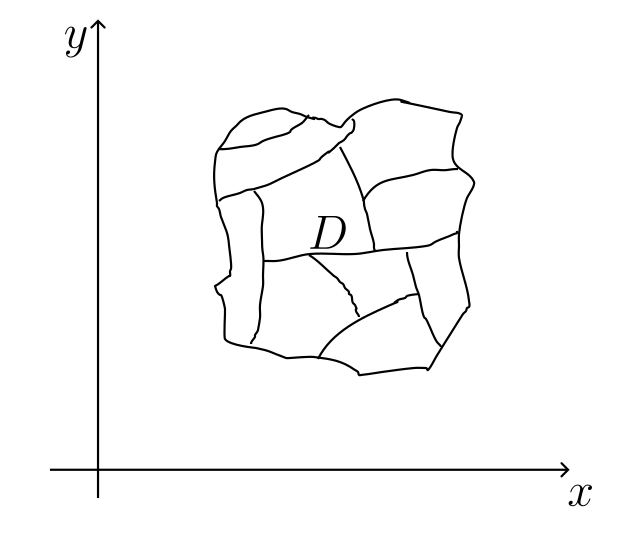
\includegraphics[scale=0.6]{8.12.2.png}
  \end{minipage}
  \hspace{1em}
  \begin{minipage}{0.55\textwidth}
    \begin{enumerate}
      \item Разобьем D спрямляемыми кривыми(кривая имеющая конечную длину)
      \item Выберем (.) $((\xi_i;\eta_i)) \in D_i$
      \item Вычислим $f((\xi_i;\eta_i))\Delta D_i$
      \item Составим $\sigma_R=\sum_{i=0}^{n-1}f((\xi_i;\eta_i))\Delta D_i$
      \item Пусть $\lambda_R = \underset{M_1,M_2 \in D_i}{\max \rho(M_1,M_2)}$
      \item Вычислим $\lim_{\lambda_R \to 0}\sigma_R=\iint_{D}f(x;y)dxdy$
    \end{enumerate}
  \end{minipage}
  \vspace{1em}
  \break
  \underline{Определение: } Если существует конечный предел $\sigma_R$, при $\lambda_R \to 0$, не
  зависящий от способа разбиения области D и выбора (.) $(\xi_i;\eta_i)$, то он называется двойным
  интегралом от функции f(x;y) по области D\\
  \subsection*{Свойства:}
  \begin{enumerate}
    \item $\iint_D dxdy=S_p$
    \item Пусть $D=D_1 \lor D_2: D_1\land D_2 =0$\\
    Если f(x;y) интегрируема в D, то она интегрируема в $D_1$ и $D_2$
    \[\iint_D f(x;y) dxdy=\iint_{D_1}f(x;y)dxdy+\iint_{D_2}f(x;y)dxdy\]
    \item Если f и g интегрируемы в D, то существует 
    \[\iint_D [\alpha f(x;y)+ \beta g(x;y)]dxdy=\alpha \iint_D f(x;y)dxdy+ \beta \iint_D g(x;y)dxdy\]
    \item Пусть f,g $\geq 0$ в D и $\forall (.) (x;y) \in D f\leq g$\\
    \[\iint_D f(x;y)dxdy\leq \iint_D g(x;y)dxdy\]
    \item Пусть f>0 $D_1 \subset D_2$
    \[\iint_{D_1} f(x;y)dxdy<\iint_{D_2} f(x;y)dxdy\]
    \item Если f интегрируема в D, то |f| тоже интегрируема в D
    \[\Big| \iint_D f(x;y)dxdy \Big| \leq \iint|f(x;y)|dxdy\]
    \item  
    \subsubsection*{Теорема о среднем}\label{th:8.12.1}
    \par\noindent
    Пусть f и g ограничены и интегрируемы в D, g не меняет знак в D
    \[m\leq f(x;y)\leq M. \text{ Тогда существует }\lambda: m\leq \lambda \leq M: 
    \iint_D f(x;y) g(x;y)dxdy=\lambda \iint_D g(x;y)dxdy\]\\
    Если дополнить f(x;y) непрерывна в D, то существует
    \[(.) (\xi_i;\eta_i) \in D: \iint_D f(x;y)dxdy=f (\xi_i;\eta_i) \Delta D\]
  \end{enumerate}
  \subsection{Вычисление двойного интеграла(сведение двойного интеграла к повторному)}
  Пусть f(x;y) задана в P = [a;b]x[c;d]. $\hspace{20pt}$ Рассмотрим F(x)=$\int_{a}^{c}f(x;y)dy$
  \subsubsection*{Теорема 8.13.1}\label{th:8.13.1}
  \par\noindent
  Если f(x;y) непрерывна в P, то F(x) непрерывна на [a;b]\\
  \underline{Доказательство:}
  \begin{adjustwidth}{1.5em}{1.5em}
    Рассмотрим $F(x+\Delta x)-F(x)=\int_{c}^{d}[f(x+\Delta x)-f(x;y)]dy \hspace{20pt} x,x+\Delta x \in [a;b]$\\
    По условию f(x;y) непрерывна в P $\Rightarrow f(x;y)$ будет равномерно непрерывна в P. \[\forall f(x;y)
    ,(x+\Delta x;y)\in P: |\Delta x|<\delta \Rightarrow |f(x+\Delta x;y)-f(x;y)|< \frac{\varepsilon}{d-c}\]\\
    То есть F(x) непрерывна в (.) x. Так как x-произвольная (.) $\in [a;b],$то F(x) непрерывна на [a;b]
    \begin{center}
      \textbf{Ч.т.д.}
    \end{center}
  \end{adjustwidth}
  \subsubsection*{Теорема 8.13.2}\label{th:8.13.2}
  \par\noindent
  Пусть $\iint_P f(x;y)dxdy$ существует. Тогда 
  \[\iint_D f(x;y)dxdy=\int_{a}^{b}dx \int_{c}^{d} f(x;y)dy=\int_{c}^{d}dy \int_{a}^{b}f(x;y)dx\]
  \underline{Доказательство:}
  \begin{adjustwidth}{1.5em}{1.5em}
    R:$\begin{cases}
      a:x_0<x_1<\dots<x_n=b & m_{ij}\leq f(x;y) \leq M_{ij} \forall (x;y) \in P_{ij} (*)\\
      c=y_0<y_1<\dots<y_k=d
    \end{cases}$\\
    Зафиксируем x=$\xi_i \in [x_i;x_{i+1}]$ и проинтегрируем (*) по переменной y
    \[\int_{y_j}^{y_{j+1}}m_{ij}dy \leq \int_{y_j}^{y_{j+1}}f(\xi_i;y)dy \leq \int_{y_j}^{y_{j+1}} M_{ij}dy\]
    \[m_{ij}\Delta y_j \leq \int_{y_j}^{y_{j+1}} f (\xi_i;y)dy \leq M_{ij}\Delta y_j\]
    \[\sum_{j=0}^{k-1} m_{ij}\Delta y_j \leq \sum_{j=0}^{k-1}\int_{y_j}^{y_{j+1}}f (\xi_i;y)dy
    \leq \sum_{j=0}^{k-1} M_{ij}\Delta y_j \Big| *\Delta x_i \text{ и проинтегрируем по } 
    i=\overline{0,n-1}\]
    \[\sum_{i=0}^{n-1}\sum_{j=0}^{k-1} m_{ij}\Delta x_j \Delta y_j \leq \sum_{i=0}^{n-1}
    [\int_{c}^{d} \equalto{f (\xi_i;y)}{I(\xi_i)}]\Delta x_i \leq 
    \sum_{i=0}^{n-1} \sum_{j=0}^{k-1} M_{ij} \Delta x_i \Delta y_j\]
    \[\text{При }\lambda_R \to 0: m_{ij},M_{ij} \rightarrow I= \iint_P f(x;y) dxdy\]
    %TODO:Найти способ как написать стрелку под текстом, пикча в Images лежит 
    Тогда $\iint_P f(x;y) dxdy = \lim_{\lambda_R \to 0} \sum_{i=0}^{n-1}I(\xi_i)\Delta x_i =
    \int_{a}^{b}I(x)dx=\int_{a}^{b}dx \int_{c}^{d}f(x;y)dy$\\
    Аналогично $\iint_P f(x;y)dxdy=\int_{c}^{d}dy \int_{a}^{b}f(x;y)dx$
    \begin{center}
      \textbf{Ч.т.д.}
    \end{center}
  \end{adjustwidth}
  \subsection{Вычисление двойного интеграла по произвольной области}
  \subsubsection*{Теорема 8.14.1}\label{th:8.14.1}
  \par\noindent
  Пусть $y_1(x)$ и $y_2(x)$ непрерывна на [a;b].\\
  Рассмотрим D:
  $\begin{cases}
    a\leq x\leq b\\
    y_1(x)\leq y \leq y_2(x)
  \end{cases}$\\
  Если f(x;y) задана в D и $\forall x \in [a;b]$ она интегрируема по y на $[y_1(x);y_2(x)]$ и
  f(x;y) непрерывна в D, то F(x) = $\int_{y_1(x)}^{y_2(x)}f(x;y)dy$ непрерывна на [a;b].\\
  \underline{Доказательство:}
  \begin{adjustwidth}{1.5em}{1.5em}
    Замена $y=y_1(x)+(y_2(x)-y_1(x))t \hspace{20pt} 0\leq t\leq 1 \hspace{20pt} dy=(y_2(x)-y_1(x))dt$
    \[F(x)=\int_{0}^{1} \underbrace{f(x;y_1(x)+(y_2(x)-y_1(x))t)(y_2(x)-y_1(x))}_{g(x;t)}dt=
    \int_{0}^{1}g(x;t)dt\]
    \begin{center}
      g(x;t) определена в прямоугольнике\\
      $a\leq x\leq b$\\
      $0\leq t\leq1$
    \end{center} 
    Тогда F(x) непрерывна по \hyperref[th:8.13.1]{Теореме 8.13.1}
    \begin{center}
      \textbf{Ч.т.д.}
    \end{center}
  \end{adjustwidth}
  \subsubsection*{Теорема 8.14.2}\label{th:8.14.2}
  \par\noindent
  Пусть f(x;y) интегрируема и непрерывна в D и $\forall x \in [a;b]$ прямая || OY пересекает границу
  D не более чем в $2^x$(.). То есть область D задана в виде D:
  $\begin{cases}
    a\leq x\leq b\\
    y_1(x)\leq y\leq y_2(x)
  \end{cases}$.\\
  Тогда:
  \[\iint_D f(x;y)dxdy = \int_{a}^{b}dx \int_{y_1(x)}^{y_2(x)}dy\]
  \underline{Замечание:} Аналогично можно рассмотреть: $\iint_D f(x;y)dxdy = \int_{c}^{d}dy
  \int_{x_1(y)}^{x_2(y)}f(x;y)dx$, если прямая || OX пересекает D не более чем в $2^x$(.).\\
  \underline{Замечание:}Если контур пересекается не более чем в $2^x$(.) как прямыми || OY,
  так и || OX, то справедливы обе формулы.\\
  \underline{Замечание:} Если контур не подходит ни под один случай, то его разбивают на $D_1,D_2,\dots$\\
  \underline{Доказательство:}
  \begin{adjustwidth}{1.5em}{1.5em}
    F(x) $\overset{\text{(на [a;b])}}{\text{непрерывна}}$ по \hyperref[th:8.14.1]{Теореме 8.14.1}. Тогда F(x)
    интегрируема на [a;b]. То есть, существует: \[\int_{a}^{b}F(x)dx=\int_{a}^{b}dx \int_{y_1(x)}^{y_2(x)}
    f(x;y)dy\]\\
    Введем разбиение:
    $\begin{cases}
      \vspace{2pt}
      x_i = a + \frac{b-a}{k}i \\
      \vspace{2pt}
      x_i-x_{i+1}=\frac{b-1}{k} \\
      i=\overline{1,k}
    \end{cases}$\\
    Введем вспомогательные функции:
    $\begin{cases}
      \vspace{2pt}
      \varphi_0(x)=y_1(x)\\
      \vspace{2pt}
      \varphi_1(x)=y_1(x)+\frac{y_2(x)-y_1(x)}{k}i\\
      \vdots\\
      \varphi_j(x)=y_1(x)+\frac{y_2(x)-y_1(x)}{k}j\\
      \vspace{2pt}
      \varphi_k(x)=y_1(x)+\frac{y_2(x)-y_1(x)}{k}k
    \end{cases}$\\
    Получим разбиение: 
    \[E^{k}_{ij}=
    \begin{cases}
      x_{i-1}\leq x \leq x_i\\
      \varphi_{j-1}\leq y\leq \varphi_j
    \end{cases} \hspace{20pt} i,j = \overline{1,k}\]
    \[m_{ij}=\underset{(x,y) \in E_{ij}^k}{\inf f(x;y)} \hspace{20pt} M_{ij}=\underset{(x,y) \in E_{ij}^k}{\sup f(x;y)}\]\\
    \[ \text{Рассмотрим} 
    \int_{a}^{b}dx+\int_{y_1(x)}^{y_2(x)}f(x;y)dy =
    \sum_{i=1}^{k} \int_{x_{i-1}}^{x_i}dx \sum_{j=1}^{k} \int_{\varphi_{j-1}}^{\varphi_j}f(x;y)dy =
    \sum_{i=1}^{k}\sum_{j=1}^{k} \int_{x_{i-1}}^{x_i} dx\int_{\varphi_{j-1}}^{\varphi_j}f(x;y)dy \leq\]
    \[\leq \sum_{i=1}^{k}\sum_{j=1}^{k} M_{ij} \int_{x_{i-1}}^{x_i}dx \int_{\varphi_{j-1}}^{\varphi_j}dy=
    \sum_{i=1}^{k}\sum_{j=1}^{k} M_{ij} M_{ij} \int_{x_{i-1}}^{x_i}dx[\varphi_j(x)-\varphi_{j_1}(x)]=
    \sum_{i=1}^{k}\sum_{j=1}^{k} \overbrace{\Delta E_{ij}^k}^{\text{S площадь}}=
    \overline{S}_R\]\\
    Аналогично $\int_{a}^{b}dx \int_{y_1(x)}^{y_2(x)}f(x;y)dy \geq \underline{S}_R$\\
    Получим $\underline{S}_R \leq \int_{a}^{b}dx \int_{y_1(x)}^{y_2(x)} f(x;y) dy \leq \overline{S}_R$
    %TODO переделать стрелки, лежит images peredelat2
    \begin{center}
      \textbf{Ч.т.д.}
    \end{center}
  \end{adjustwidth}
  \subsection{Формула Грина}
  \begin{minipage}{0.45\textwidth}
    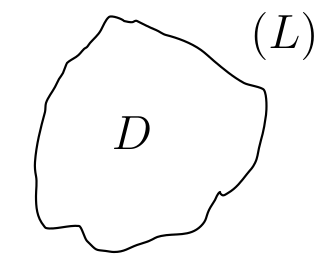
\includegraphics[scale=1]{8.15.1.png}
  \end{minipage}
  \hspace{1em}
  \begin{minipage}{0.55\textwidth}
    \[\oint_{L}Pdx+Qdy\]
  \end{minipage}
  \vspace{1em}
  \par

  \begin{minipage}{0.45\textwidth}
    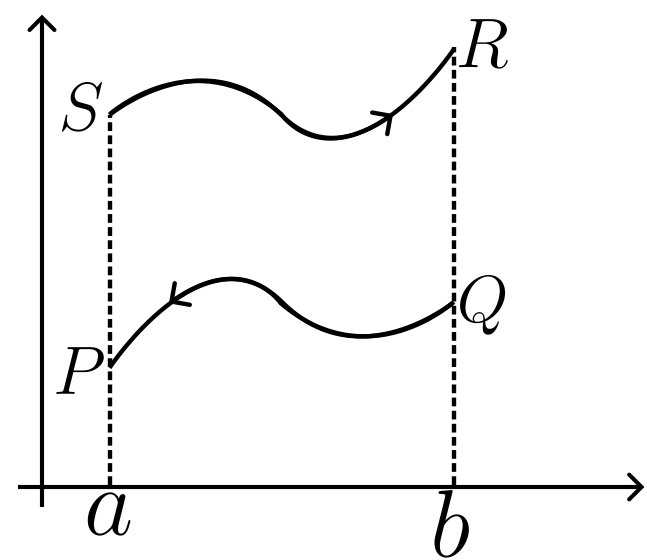
\includegraphics[scale=0.6]{8.15.2.png}
  \end{minipage}
  \hspace{1em}
  \begin{minipage}{0.55\textwidth}
    Рассмотрим 
    $\begin{cases}
      PQ:y=y_1(x)\\
      SR: y=y_2(x)\\
      a\leq x \leq b\\
      PS|OY, QR||OY
    \end{cases}$\\
  \end{minipage}
  \vspace{1em}
  \par
  Пусть в области D задана P(x;y). P(x;y) непрерывна $\frac{\delta P}{\delta y}$ непрерывна.
  \[\text{Рассмотрим }\] \[ \iint_D \frac{\delta P}{\delta y}dxdy= 
  \int_{a}^{b}dx \int_{y_1(x)}^{y_2(x)} \frac{\delta P}{\delta y}dy=
  \int_{a}^{b}dx \Big[P(x;y)\Big|_{y_1(x)}^{y_2(x)}\Big]=
  \int_{a}^{b}dx \Big[P(x;y_2(x))-P(x;y_1(x))\Big] \boxed{=}\]
  \[\text{Рассмотрим} \int_{a}^{b}P(x;y_2(x))dx=\int_{(SR)}P(x;y)dx\]
  \[\text{Рассмотрим} \int_{a}^{b}P(x;y_1(x))dx=\int_{(PQ)}P(x;y)dx=-\int_{(QP)}P(x;y)dx\]
  \[\boxed{=} \int_{(SR)}P(x;y)dx +\int_{(QP)}P(x;y)dx+\int_{(RQ)}P(x;y)dx+\int_{(PS)}P(x;y)dx \boxed{=}\]
  Пусть L-контур в положительном направлении.
  \[\boxed{=} - \int_{(L)}P(x;y)dx\]\\
  \break
  Аналогично:\\
  \par
  \begin{minipage}{0.45\textwidth}
    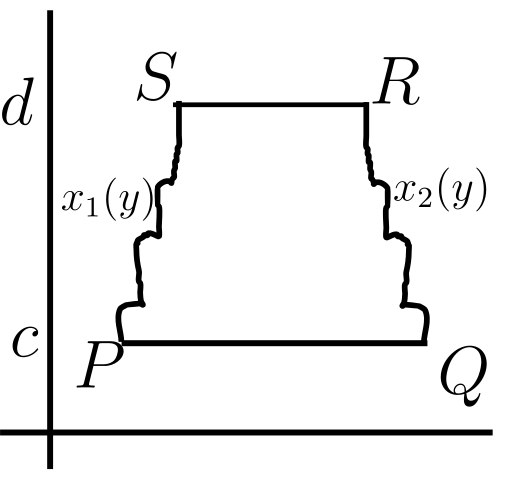
\includegraphics[scale=0.8]{8.15.3.png}
  \end{minipage}
  \hspace{1em}
  \begin{minipage}{0.55\textwidth}
    \[0,\frac{\delta Q}{\delta x} \text{непрерывна в D}\]
    \[\iint_P \frac{\delta Q}{\delta x}dxdy=\dots=\int_{(L)} Q(x;y)dy\] 
  \end{minipage}
  \vspace{1em}
  \par
  \begin{center}
    Если область D удовлетворяет обоим случаям, тогда справедлива формула:
    \[\boxed{\int_{(L)}Pdx+Qdy=\iint_D \Big[ \frac{\delta Q}{\delta x}-\frac{\delta P}{\delta y}\Big]dxdy}\]
  \end{center}
  \break
  \subsection{Замена переменных в двойном интеграле}
  \subsection*{I Преобразование плоских областей.}
  Рассмотрим 2 прямоугольных СК: xy и $\xi \eta$\\
  \begin{minipage}{0.5\textwidth}
    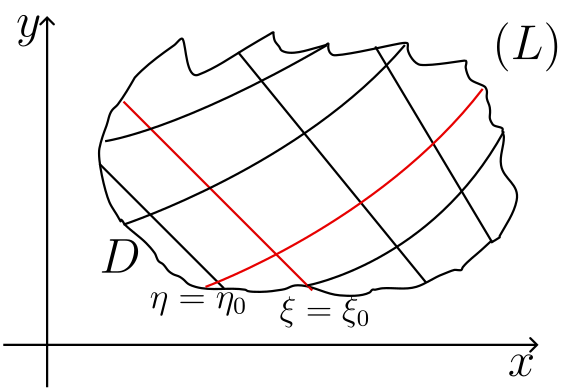
\includegraphics[scale=0.8]{8.16.1.png}
  \end{minipage}
  \hspace{1em}
  \begin{minipage}{0.5\textwidth}
    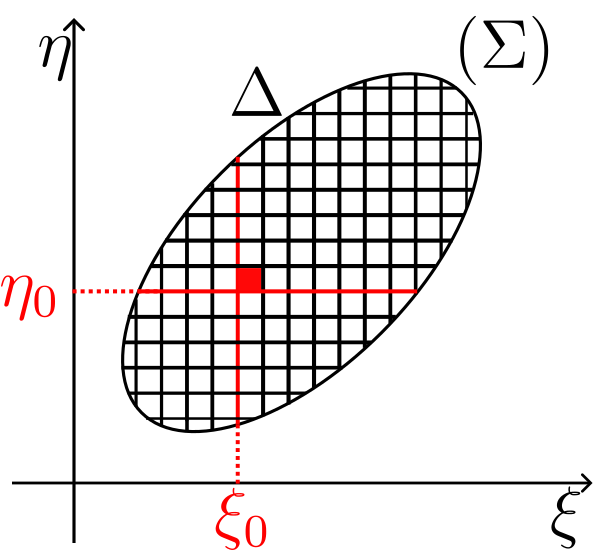
\includegraphics[scale=0.7]{8.16.2.png}
  \end{minipage}
  \vspace{1em}
  \par
  Пусть в области $\Delta$ задана системой непрерывных функций:
  $\begin{cases}
    x=x(\xi,\eta)\\
    y=y(\xi,\eta)
  \end{cases} (1)$\\
  Если различными (.) $(\xi;\eta) \in \Delta$ отвечают различные (.) $(x,y) \in D,$ то система (1)
  однозначно разрешима относительно $\xi$ и $\eta$.
  $\begin{cases}
    \xi=\xi(x;y)\\
    \eta=\eta(x;y)
  \end{cases} (2)$\\
  \underline{Определение: } $\frac{D(x;y)}{D(\xi,\eta)}=
  \begin{vmatrix}
    \frac{\delta x}{\delta \xi} & \frac{\delta x}{\delta \eta}\\
    \frac{\delta y}{\delta \xi} & \frac{\delta y}{\delta \eta}
  \end{vmatrix}$ Якобиан перехода из КСК в ДСК.\\
  \begin{itemize}
    \item Если $\frac{D(x;y)}{D(\xi;\eta)} \not = 0,$ то внутренней (.) $\xi,\eta$ соответствует
    внутренней (.) (x;y).\\Граничной (.) $(\xi,\eta)$ соответствует граничная (.) $(x;y)$
    \item Если $\frac{D(x;y)}{D(\xi;\eta)} > 0$, то при переходе в ДСК, направление обхода не меняется.
    \item Если $\frac{D(x;y)}{D(\xi;\eta)} < 0$, то при переходе в ДСК, направление обхода поменяется.
    \item Если в $\Delta$ взять гладкую кривую, то с помощью (1):
    $\begin{matrix}
        \begin{cases}
          \xi=\xi(t)\\
          \eta=\eta(t)
        \end{cases} \alpha\leq t\leq\beta\\
        \begin{cases}
          x=x(\xi(t);\eta(t))=x(t)\\
          y=y(\xi(t);\eta(t))=y(t)
        \end{cases} (3)
      \end{matrix}$
  \end{itemize}
  \underline{Примеры:}\\
  a)ПСК
  \[\begin{matrix}
    x=r\cos(\varphi) & r=\sqrt{x^2+y^2}\\
    y=r\sin(\varphi) & \varphi=
    \begin{cases}
      \arcctg \frac{y}{x},(.) (x;y) \in \text{ I, II ч.}\\
      \arcctg \frac{y}{x}+\pi,(.) (x;y) \in  \text{II,III ч.}\\
    \end{cases}
  \end{matrix}\]\\
  \break
  б) Семейство пересекающих парабол.
  \[y^2 =2px \hspace{20pt} x^2=2qy\] 
  \begin{minipage}{0.45\textwidth}
    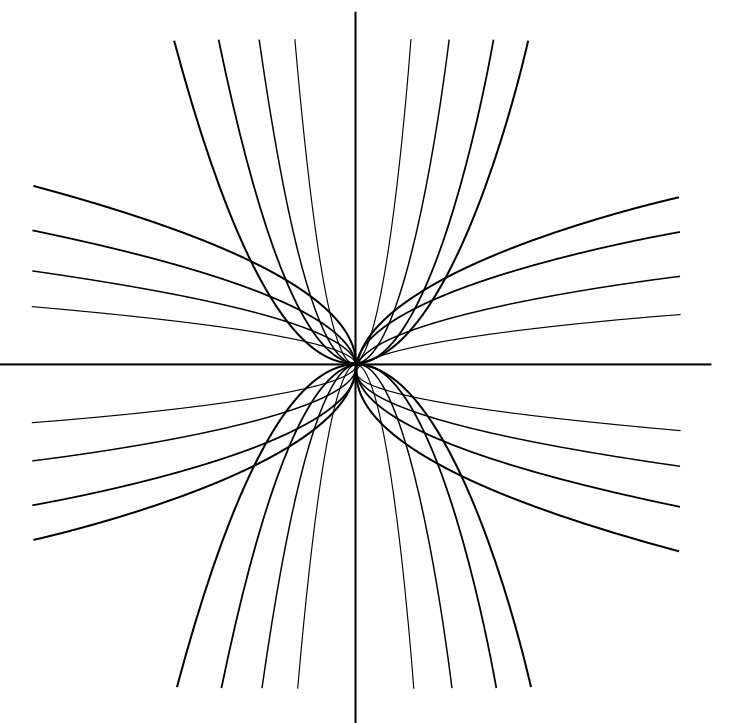
\includegraphics[scale=0.6]{8.16.3.png}
  \end{minipage}
  \hspace{1em}
  \begin{minipage}{0.55\textwidth}
    $\text{ Пусть } 2p=\xi \hspace{20pt} 2q=\eta$\\
    $y^2=\xi x \hspace{20pt} x^2=\eta y$\\
    $x^4=\eta^2y^2=\eta^2 \xi x$\\
    $x^3=\eta^2 \xi$\\
    $\begin{vmatrix}
      x=\sqrt[3]{\eta^2 \xi}\\
      y=\sqrt[3]{\xi^2 \eta}
    \end{vmatrix} 
    \begin{matrix}
      \xi=\frac{x}{y^2}\\
      \eta=\frac{y}{x^2}
    \end{matrix}$
  \end{minipage}
  \vspace{1em}
  \par
  \subsection*{II Вычисление площади в криволинейной системе координат:}
  Рассмотри область $D \in x;y,$ ограниченную кусочно-гладкую контуром L. Пусть существует (1) и (2).
  Пусть существует $\frac{\delta^2 y}{\delta \xi \delta \eta}$ и она непрерывна. Найти $S_D$.\\
  \[S_D =\int_{(L)}xdy=
  \begin{vmatrix}
    x=x(t)\\
    y=y(t)\\
    \alpha \leq t \leq \beta\\
    \text{\underline{Замечание:} при изменении t от } \alpha \text{ до } \beta\\
     \text{L - положительный контур.}
  \end{vmatrix} 
  = \int_{a}^{b} x(t)y'(t)dt \overset{(3)}{=} \] 
  \[\overset{(3)}{=} \int_{\alpha}^{\beta} x(\xi(t),\eta(t))
  \Big[ \frac{\delta y}{\delta \xi}\xi'(t)+\frac{\delta y}{\delta \eta}\eta'(t)\Big]dt \boxed{=}\]\\
  Рассмотрим $\int_{\Sigma} x(\xi;\eta) \Big[\frac{\delta y}{\delta\xi}d\xi + \frac{\delta y}{\delta \eta}d \eta\Big]
  \rightarrow \int_{\alpha}^{\beta}x(\xi(t);\eta(t))\Big[ \frac{\delta y}{\delta \xi} \xi'(t)+
  \frac{\delta y}{\delta \eta}\eta'(t)\Big]dt$\\
  \[\boxed{=} \pm \int_{\Sigma}x(\xi(t);\eta(t)) \Big[\frac{\delta y}{\delta\xi}d\xi + \frac{\delta y}{\delta \eta}d \eta\Big]
  \boxed{=}
  \begin{matrix}
    \text{"+", если положительный обход у L соответствует} \\
    \text{положительному обходу } \Sigma\\
    \text{"-", если положительный обход у L соответствует} \\
    \text{отрицательному обходу } \Sigma
  \end{matrix}\]
  \begin{center}
    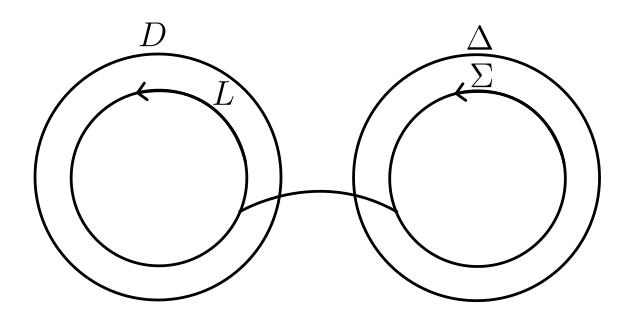
\includegraphics[scale=0.7]{8.16.4.png}
  \end{center}
  \subsection*{Формула Грина:}
  \[\int_{(L)} Pdx+Qdy=\iint_D \Big[ \frac{\delta Q}{\delta x} - \frac{\delta P}{\delta y}\Big] dxdy\]
  \[\int_{(\Sigma)}P(\xi;\eta)d\xi+Q(\xi;\eta)d\eta= \iint_{\Delta} \Big[\frac{\delta Q}{\delta \xi} -\frac{\delta P}{\delta \eta} d\xi d\eta \Big]\]
  \[P(\xi;\eta)=x \frac{\delta y}{\delta \xi} \hspace{20pt} Q(\xi;\eta)=x \frac{\delta y}{\delta \eta}\]
  \[\frac{\delta Q}{\delta \xi}=\frac{\delta}{\delta \xi}(x \frac{\delta y}{\delta \eta})=
  \frac{\delta x}{\delta \xi}\frac{\delta y}{\delta \eta}+x\frac{\delta^2y}{\delta\xi \delta\eta}\]
  \[\frac{\delta P}{\delta \eta}=\frac{\delta}{\delta \eta}(x \frac{\delta y}{\delta \xi})=
  \frac{\delta x}{\delta \eta} \frac{\delta y}{\delta \xi}+x \frac{\delta^2 y}{\delta \eta \delta \xi}\]
  \[\frac{\delta Q}{\delta \xi}-\frac{\delta P}{\delta \eta}=\frac{\delta x}{\delta \xi} \frac{\delta y}{\delta \eta}-
  \frac{\delta x}{\delta \eta}\frac{\delta y}{\delta \xi}=
  \begin{vmatrix}
    \frac{\delta x}{\delta \xi} & \frac{\delta x}{\delta \eta}\\
    \frac{\delta y}{\delta \xi} & \frac{\delta y}{\delta \eta}\\
  \end{vmatrix} = \frac{D(x;y)}{D(\xi;\eta)}\]\\
  \[\boxed{=} \pm \iint_\Delta \frac{D(x;y)}{D(\xi;\eta)}d\xi d\eta \overset{\text{опр Якобиана}}{=} 
  \underbracket{\iint_\Delta \Big|\frac{D(x;y)}{D(\xi;\eta)}\Big|d\xi d\eta \boxed{=}}\]
  Теорема Лагранжа:
  \[f(b)-f(a)=f'(\xi)(b-a) \hspace{20pt} 
  \begin{matrix}
    \varepsilon = f'(\xi)\delta\\
    \lim_{\lambda_R \to 0} \frac{\varepsilon}{\delta}=f'(\xi)
  \end{matrix} \hspace{20pt} f'(\xi)=\frac{\varepsilon}{\delta}\]
  $f'(\xi)$ является коэффициентом растяжение(сжатия) прямой x в прямоугольнике в данной её (.)($\xi$)\\
  \[\overset{\hyperref[th:8.12.1]{\text{Теорема о среднем}}}{\boxed{=}}
  \Big|\frac{D(x;y)}{D(\xi;\eta)} \Big|_{M \in \Delta} \hspace{20pt} S_\Delta=S_D\]
  \[\iint_D f(x;y)dxdy=f(\xi;\eta)\iint_D dxdy = f(\xi;\eta)S_D\]
  \[\Big| \frac{D(x;y)}{D(\xi;\eta)}\Big|_{M \in \Delta} = \lim_{\Delta \to M} \frac{S_D}{S_\Delta}\]
  Модуль величины Якобиана в (.) есть коэффициент растяжения (сжатия) плоскости $\xi \eta$ при преобразовании
  её в плоскость $xy$
  \subsection*{III Замена переменных в двойном интеграле:}
  Рассмотрим $\iint_{D} f(x;y)dxdy$\\
  \begin{enumerate}
    \item Разбиваем область D кусочно-гладкими кривыми
    \item Разбиение R и так далее
  \end{enumerate}
  \[\sigma_R = \sum_{i=0}^{n-1} f(x_i;y_i)S_{D_i} =\sum_{i=0}^{n-1} f(x_i;y_i) \Big| I \Big| \Big|_{\overline{M_i}(\xi_i;\eta_i)}
  * S_{\Delta_i} \boxed{=} \]
  \begin{center}
    Так как $(x_i;y_i)$ - произвольная (.), то выберем её так\\ 
    чтобы в области $D_i$ ей соответствовала (.) $(\overline{\xi_i};\overline{\eta_i})$ в $\Delta_i$
  \end{center}
  \[\boxed{=} \sum_{i=0}^{n-1} f(x(\overline{\xi_i},\overline{\eta_i});y(\overline{\xi_i},\overline{\eta_i}))
  |I|_{\overline{M_i}(\xi_i;\eta_i)}S_{\Delta_i}\]
  \[\lim_{\lambda_R \to 0} \sigma_R \iint_D f(x(\xi;\eta);y(\xi;\eta))|I|d\xi d\eta\]
  Для ПСК: 
  $
  \begin{matrix}
    x=r\cos\varphi\\
    y=r\sin\varphi
  \end{matrix} \hspace{20pt}
  I = \begin{vmatrix}
    \frac{\delta x}{\delta r} & \frac{\delta x}{\delta \varphi}\\
    \frac{\delta y}{\delta r} & \frac{\delta y}{\delta \varphi}
  \end{vmatrix}=
  \begin{vmatrix}
    \cos\varphi & -r\sin\varphi\\
    \sin \varphi & r\cos\varphi 
  \end{vmatrix} = r\cos^2\varphi+r\sin^2\varphi=r
  $
  \[|I|=r\]
  \subsection{Приложения двойных интегралов.}
  \begin{enumerate}
    \item \[S_D=\iint_D dxdy\]
    \item \[V=\iint_D f(x;y)dxdy=\iint_{\overline{D}} f(x;z)dxdz = \iint_{\overline{\overline{D}}}f(y;z) dydz
    =\iint_{\overline{\overline{\overline{D}}}}F(x(u;v);y(u;v);z(u;v))dudv\]
    \item \[m=\iint_D \underbrace{\rho}_{\frac{kg}{m^2}}dxdy\]
    \item \[
    \begin{matrix}
      M_x=\iint \rho y dxdy & M_y=\iint_{\rho}\rho xdxdy\\
      x_c=\frac{M_y}{m} & y_c=\frac{M_x}{m}
    \end{matrix}\]
  \end{enumerate}
  \subsection{Площадь поверхности.}
  Пусть $Z=f(x;y)$. Можно говорить о верхней и нижней стороне поверхности. Если поверхность замкнута,
  то можно говорить о внешней стороне поверхности и о внутренней. Возьмём на поверхности произвольную
  (.) $m_0$, проведем в ней нормаль. И проведем из (.) $m_0$ замкнутый контур, начиная и заканчивая 
  в (.) $m_0$(при этом нормаль изменяется непрерывно). При возврате в (.) $m_0$ можно получить 2 
  варианта: 
  \begin{enumerate}
    \item вектор нормали сохранил своё направление;
    \item вектор нормаль поменяет непрерывные на противоположные.
  \end{enumerate}
  \underline{Определение: } Если при обходе по контуру нормаль меняет направление на противоположное,
  то поверхность называется односторонней. Если не поменяет по замкнутому контуру - двусторонней.\\
  \begin{minipage}{0.54\textwidth}
    \underline{Пример:} лист Мёбиуса - односторонняя поверхность. 
  \end{minipage}
  \hspace{1em}
  \begin{minipage}{0.3\textwidth}
    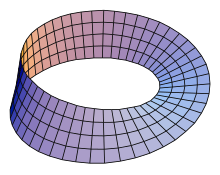
\includegraphics[scale=1]{8.18.1.png}
  \end{minipage}
  \vspace{1em}
  \par
  \underline{Определение: } Совокупность всех (.) поверхности с приписанными в них направлениями 
  нормалей называется стороной поверхности.\\
  \underline{Ориентация поверхностей}: 
  \begin{itemize}
    \item Верхняя сторона поверхности (острый угол с осью $OZ$) и замкнутую поверхность (внешняя сторона) 
    будем считать положительно ориентированными(правая ориентация)
    \item Нижняя сторона поверхности или внутренняя сторона(замкнутая поверхность) будем считать
    отрицательной ориентацией(левая ориентация)
  \end{itemize}
  \underline{Площадь поверхности}: Рассмотрим не замкнутую гладкую поверхность $S$, ограниченную
  кусочно-гладким контуром L.\\
  Разложим эту поверхность на элементарные $S_1,\dots,S_n$\\
  В каждой элементарной $S_i$ выберем произвольную (.) $M_i$ и в этой (.) проведем касательную
  плоскость к $S_i$\\
  \par
  \begin{minipage}{0.45\textwidth}
    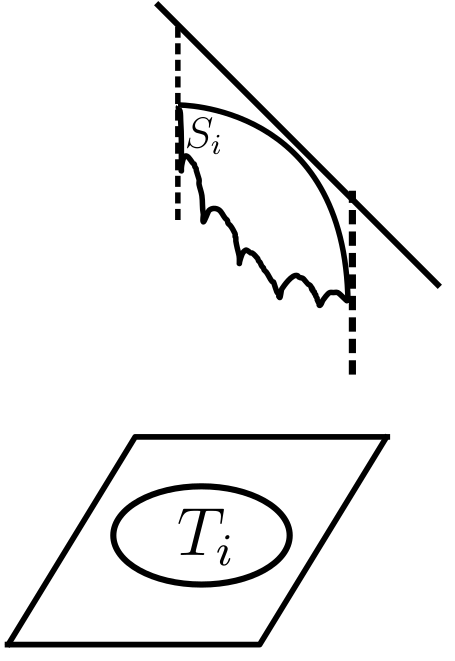
\includegraphics[scale=0.6]{8.18.2.png}
  \end{minipage}
  \hspace{1em}
  \begin{minipage}{0.55\textwidth}
    Построим на границе области $S_i$ цилиндрическую поверхность с образующими || оси OZ.Пересечение
    этого цилиндра с касательной плоскостью образует плоскую фигуру $T_i$.
    \[\text{Тогда }S=\lim_{\lambda_R \to 0} \Sigma \Delta T_i\]
  \end{minipage}
  \vspace{1em}
  \par
  Пусть поверхность задана:
  \[
  \begin{matrix}
    x=x(u;v)\\
    y=y(u;v)\\
    z=z(u;v)
  \end{matrix} \hspace{20pt}
  \begin{cases}
    x=r\cos(u)\\
    y=r\sin(u)\\
    z=v
  \end{cases} \text{ - цилиндрическая поверхность}
  \]
  Пусть $\mu' \in S \hspace{20pt} \mu'(x';y';z')$. Пересечем СК в (.) $\mu'$ и перейдем к новой
  СК $\xi \eta \chi$.\\
  \break
  \underline{Формулы преобразования координат:}
  \[\xi=(x-x')\cos(\alpha_1)+(y-y')\cos(\beta_1)+(z-z')\cos(\gamma_1)\]
  \[\eta=(x-x')\cos(\alpha_2)+(y-y')\cos(\beta_2)+(z-z')\cos(\gamma_2)\]
  \[\chi=(x-x')\cos(\alpha_3)+(y-y')\cos(\beta_3)+(z-z')\cos(\gamma_3)\]
  \begin{tabular}{ p{10pt}|p{10pt}|p{10pt}|p{10pt} }
    & X & Y & Z\\
    \hline
    $\xi$ & $\alpha_1$ & $\beta_1$ & $\gamma_1$\\
    \hline
    $\xi$ & $\alpha_2$ & $\beta_2$ & $\gamma_2$\\
    \hline
    $\xi$ & $\alpha$ & $\beta$ & $\gamma$\\
  \end{tabular}
  \hspace{20pt} $T_i = \iint_{D_{UV}}dudv=\iint_{D_{\xi \eta}}\Big| \frac{D(\xi;\eta)}{D(u;v)}\Big|
  d \xi d \eta$
  \[\frac{D(\xi;\eta)}{D(u;v)}=
  \begin{vmatrix}
    \frac{\delta \xi}{\delta u} &\frac{\delta \xi}{\delta V}\\
    \frac{\delta\eta}{\delta u} &\frac{\delta \eta}{\delta V}
  \end{vmatrix}=
  \]
  \[=\Big|
  \begin{matrix}
  \frac{\delta \xi}{\delta x}\frac{\delta x}{\delta u}+\frac{\delta \xi}{\delta y}\frac{\delta y}{\delta u}+
  \frac{\delta \xi}{\delta z}\frac{\delta Z}{\delta u} = x'_u\cos(\alpha_1)+y'_u\cos(\beta_1)+z'_u\cos(\gamma_1) & x'_u\cos(\alpha_1)+y'_u\cos(\beta_1)+z'_u\cos(\gamma_1) \\
  x'_v\cos(\alpha_2)+y'_v\cos(\beta_2)+z'_v\cos(\gamma_2) & x'_v\cos(\alpha_2)+y'_v\cos(\beta_2)+z'_v\cos(\gamma_2) 
  \end{matrix}\Big| =
  \]
  \[\begin{vmatrix}
    \begin{pmatrix}
      x'_u & y'_u & z'_u\\
      x'_v & y'_v & z'_v
    \end{pmatrix}
    \begin{pmatrix}
      \cos(\alpha_1)& \cos(\alpha_2)\\
      \cos(\beta_1)&\cos(\beta_2)\\
      \cos(\gamma_1)&\cos(\gamma_2)
    \end{pmatrix}
  \end{vmatrix}=\]
  \[=\underbrace{\begin{vmatrix}
    y'_u & z'_u\\
    y'_v & z'_v
  \end{vmatrix}}_{A}
  \underbrace{\begin{vmatrix}
    \cos(\beta_1) & \cos(\gamma_1)\\
    \cos(\beta_2) & \cos(\gamma_2)
  \end{vmatrix}}_{\cos(\alpha)}
  +
  \underbrace{\begin{vmatrix}
    z'_u&x'_u\\
    z'_v&x'_v
  \end{vmatrix}}_{B}
  \underbrace{\begin{vmatrix}
    \cos(\gamma_1) & \cos(\alpha_1)\\
    \cos(\gamma_2)&\cos(\alpha_2)
  \end{vmatrix}}_{\cos(\beta)}
  +
  \underbrace{\begin{vmatrix}
    x'_u & y'_u\\
    x'_v & y'_v
  \end{vmatrix}}_{C}
  \underbrace{\begin{vmatrix}
    \cos(\alpha_1)&\cos(\beta_1)\\
    \cos(\alpha_2)&\cos(\beta_2)
  \end{vmatrix}}_{\cos(\gamma)}
  \boxed{=}\]
  \par
  \underline{Замечание:} Каждый из координатных ортов ($\overline{\cos(\alpha_1);\cos(\beta_1);\cos(\gamma_1)}$),($\overline{\cos(\alpha_2);\cos(\beta_2);\cos(\gamma_2)}$)
  ,($\overline{\cos(\alpha);\cos(\beta);\cos(\gamma)}$) взаимно перпендикулярны.
  Поэтому:
  \[(\overline{\cos(\alpha);\cos(\beta);\cos(\gamma)}) = 
  \begin{vmatrix}
    i&j&k\\
    \cos(\alpha_1)&\cos(\beta_1)&\cos(\gamma_1)\\
    \cos(\alpha_2)&\cos(\beta_2)&\cos(\gamma_2)
  \end{vmatrix}=\]
  \[= \overline{i}
  \equalto{
    \begin{vmatrix}
    \cos(\beta_1)&\cos(\gamma_1)\\
    \cos(\beta_2)&\cos(\gamma_2)
    \end{vmatrix}
  }{\cos(\alpha)}+ \overline{j}
  \begin{vmatrix}
    \cos(\alpha_1)&\cos(\gamma_1)\\
    \cos(\alpha_2)&\cos(\gamma_2)
  \end{vmatrix}
  + \overline{k}
  \begin{vmatrix}
    \cos(\alpha_1)&\cos(\beta_1)\\
    \cos(\alpha_2)&\cos(\beta_2)
  \end{vmatrix}
  \]
  \[\boxed{=}A\cos(\alpha)+B\cos(\beta)+C\cos(\gamma)\boxed{=}\]
  \underline{Определение: } Если поверхность задана $\begin{matrix}
    x=x(u;v)\\
    y=y(u;v)\\
    z=z(u;v)
  \end{matrix}$, то нормаль к поверхности задается$\begin{vmatrix}
    \overline{i}&\overline{j}&\overline{k}\\
    x'_u & y'_u & z'_u\\
    x'_v & y'_v & z'_v
  \end{vmatrix}=(n_x;n_y;n_z)=\overline{(A;B;C)}$\\
  \underline{Пример:}\\
  \[\begin{matrix}
    \text{Рассмотрим } z=f(x;y)\\
    u=x\\
    v=y
  \end{matrix}
  \hspace{20pt}
  \begin{vmatrix}
    \overline{i}&\overline{j}&\overline{k}\\
    1&0&z'_x\\
    0&1&z'_y 
  \end{vmatrix}=
  \begin{matrix}
    \overline{i}(-z'_x)-jz'_y+\overline{k}\\
    (-z'_x;-z'_y;1) \text{ или }\\
    (z'_x;z'_y;-1)
  \end{matrix}\]
  \underline{С другой стороны:}
  \[
  \cos(\alpha)=\frac{A}{\pm \sqrt{A^2+B^2+C^2}}\\
  \cos(\beta)=\frac{B}{\pm \sqrt{A^2+B^2+C^2}}\\
  \cos(\gamma)=\frac{C}{\pm \sqrt{A^2+B^2+C^2}}
  \]
  Пусть $A',B',C'$ - значения определителей $A,B,C$ в (.) $\mu'$
  \[\boxed{=}
  \frac{AA'+BB'+CC'}{\pm \sqrt{A^2+B^2+C^2}}
  \boxed{=}\]
  Если расстояние между (.) ($u;v$) и ($u';v'$) стремится к нулю, то $\frac{D(\xi;\eta)}{D(u;v)} = \sqrt{A'^2+B'^2+C'^2}+\varepsilon'$
  \[
  S_{T_i}=\iint_{D_{uv}}\sqrt{A^2+B^2+C^2}dudv+\varepsilon;S_\text{поверхности}=\lim_{\lambda_R \to 0}\Sigma S_{T_i}=\iint_{D_{uv}}\sqrt{A^2+B^2+C^2}dudv=S
  \]
  \[
  \text{Рассмотрим }
  \begin{pmatrix}
    x_u & y'_u &z'_u\\
    x'_v&y'_v&z'_v
  \end{pmatrix}
  \begin{pmatrix}
    x'_u &x'_v\\
    y'_u&y'_v\\
    z'_u&z'_v
  \end{pmatrix}
  =
  \begin{pmatrix}
    x'^2_u+y'^2_u+z'^2_u & x'_u x'_v+y'_u y'_v+ z'_u z'_v\\
    \underbrace{x'_u x'_v+y'_u y'_v+ z'_u z'_v}_F & \underbrace{x'^2_v+y'^2_v+z'^2_v}_{G}
  \end{pmatrix}
  \]
  \[
  \text{Рассмотрим } \begin{vmatrix}
    E & F\\
    F & G
  \end{vmatrix} =EG-F^2=A^2+B^2+C^2 \hspace{20pt} S=\iint_{D_{uv}}\sqrt{EG-F^2}dudv
  \]
  $\text{Рассмотрим } Z=f(x;y) \text{ уравнение поверхности}.
  \begin{matrix}
    u \sim x\\
    v \sim y
  \end{matrix}$ 
  \[ A=
  \begin{vmatrix}
    y'_u & z'_u \\
    y'_v & z'_v
  \end{vmatrix} =\begin{vmatrix}
    0 & z'_x\\
    1 & z'_y
  \end{vmatrix}=-z'_x\]
  \[ B=
  \begin{vmatrix}
    z'_u & x'_u \\
    z'_v & x'_v
  \end{vmatrix} =\begin{vmatrix}
    z'_x & 1\\
    z'_y & 0
  \end{vmatrix}=-z'_y\]
  \[ C=
  \begin{vmatrix}
    x'_u & y'_x\\
    x'_v & y'_y
  \end{vmatrix} =\begin{vmatrix}
    1 & 0\\
    0 & 1
  \end{vmatrix}=1\]
  \[S=\iint_{D_{xy}}\sqrt{1 + z'^2_x + z'^2_y}dxdy\]
  Рассмотрим $\cos(\gamma)=\frac{C}{\pm \sqrt{A^2+B^2+C^2}}=\frac{1}{\pm \sqrt{1+z'^2_x+z'^2_y}}$
  \[S=\iint_{D_{xy}}\sqrt{1+z'^2_x+z'^2_y}dxdy=\iint_{D_{xy}}\frac{dxdy}{|\cos(\gamma)|} \hspace{20pt} \gamma - \forall \text{ угол}\]
  \break
  \subsection{Поверхностные интегралы I и II рода.}
  Пусть в каждой (.) двусторонней гладкой(или кусочно-гладкой) поверхности, ограниченной кусочно-гладким контуром
  определена функция f(x;y;z)
  \begin{enumerate}
    \item Производим разбиение R поверхности
    \item Выберем (.) $\mu_i$ произвольно: $\mu_i \in S_i$
    \item Вычислим $f(\mu_i) = f(x_i;y_i;z_i)$
    \item Вычислим $f(x_i;y_i;z_i)\Delta S_i$
    \item Составим $\sigma_R=\sum_{i=0}^{n-1}f(x_i;y_i;z_i)\Delta S_i$
    \item Вычислим $\lim_{\lambda_R \to 0} \sigma_R = \iint_{S} f(x;y;z)dS$
  \end{enumerate}
  \underline{Определение: }Если существует конечный $\lim_{\lambda_R \to 0}$, не зависящий от способа разбиения поверхности
  S и выбора (.) $\mu_i$ , то он называется поверхностным интегралом I рода от функции $f(x;y;z)$ по поверхности S.\\
  \underline{Вычисление: } 
  \[ \iint_S f(x;y;z)dS=\iint_{D_{xy}}f(x;y;z(x;y)) \sqrt{1+z'^2_x+z'^2_y}dxdy = 
  \iint_{D_{uv}} f(x(u;v);y(u;v);z(u;v))\sqrt{EG-F^2}dudv\]
  \subsection*{Поверхностные интегралы II рода:}
  Пусть в каждой (.) двусторонней гладкой(или кусочно-гладкой) поверхности, ограниченной кусочно-гладким контуром
  определена функция $f(x;y;z)$.\\ Выберем одну из сторон поверхности:
  \begin{enumerate}
    \item Произведем разбиение R к поверхности
    \item Выберем (.) $\mu_i$ произвольно: $\mu_i \in S_i$
    \item Вычислим $f(\mu_i)=f(x;y;z)$
    \item Вычислим $f(x_i;y_i;z_i)\Delta D_i; \hspace{20pt} \Delta D_i$ - проекция $S_i$ на плоскость $Dy$\\
    Проекция берется со знаком "+", если вектор нормали к поверхности образует острый угол с осью $OZ$. "-" если угол
    между нормалью и $OZ$ тупой.
    \item Составим $\sigma_R=\sum_{i=0}^{n-1}f(x_i;y_i;z_i)\Delta D_i$
    \item $\lim_{\lambda_R \to 0}\sigma_R=\iint_S f(x;y;z)dxdy$
  \end{enumerate}
  \underline{Определение: }  Если существует конечный $\lim_{\lambda_R \to 0}$, не зависящий от способа разбиения
  поверхности S и выбора (.) $\mu_i$, то он называется поверхностным интегралом II рода от функции $f(x;y;z)$ по 
  поверхности S.\\
   \[\text{Аналогично: }\iint_S f(x;y;z)dxdz, \iint_S f(x;y;z)dydz\]
  \[\iint_S P(x;y;z)dydz+Q(x;y;z)dxdz+R(x;y;z)dxdy\text{ - поверхностный интеграл II рода общего вида}\]
  \underline{Вычисление: }
  \[\iint_S f(x;y;z)dxdy = \pm \iint_{D_{xy}} f(x;y;z(x;y))dxdy\]
  \pagebreak
  \subsection{Связь между поверхностными интегралами I и II рода.}
  Рассмотрим $\sigma_R=\sum_{i=1}^{n} f(x_i;y_i;z_i)\Delta D_i$\\
  Рассмотрим $\Delta S_i = \iint_D \frac{dxdy}{\cos(\gamma_i)} \hspace{20pt} \gamma_i$- острый угол\\
  \underline{Применим \hyperref[th:8.12.1]{теорему о среднем}}:
  \[\Delta S_i = \frac{1}{\cos(\overline{\gamma_i})}\iint_{D_i} dxdy= \frac{1}{\cos(\overline{\gamma_i})}\Delta D_i
  \Rightarrow \Delta D_i = \cos(\overline{\gamma_i})\Delta S_i\]
  Тогда $\sigma_R=\sum_{i=1}^{n}f(x_i;y_i;z_i)\cos(\overline{\gamma_i})\Delta S_i.\sigma_R$ не является интегральной суммой
  (зависит не от одной(.)).\\
  Рассмотрим $\sigma_R^*=\sum_{i=1}^{n}f(x_i;y_i;z_i)\cos(\overline{\gamma_i})\Delta S_i$. \\
  Оценим $|\sigma_R-\sigma_R^*|= \sum_{i=1}^{n}f(x_i;y_i;z_i)|\cos(\gamma_i)-\cos(\overline{\gamma_i})|\Delta S_i \boxed{<}$
  \begin{enumerate}
    \item $f(x;y;z)$ интегрируема $\Rightarrow$ она ограниченна в каждой (.) поверхности S.
    \[|f(x_i;y_i;z_i)|<M_i\]
    \item Функция $\cos(\gamma)$ непрерывна, т.е.:
    \[\Delta S_i < \delta \Rightarrow |\cos(\gamma_i)-\cos(\overline{\gamma_i})|<\varepsilon\]
  \end{enumerate}
  \boxed{<} $M\varepsilon \Delta S =\varepsilon^*$
  \[\lim_{\lambda_R \to 0} \sigma_R = \lim_{\lambda_R \to 0} \sigma_R^* = \iint_S f(x;y;z)\cos(\gamma)dS\]
  \underline{Замечание:} $\iint_{S} f(x;y;z)dxdy \boxed{=} $ S - цилиндрическая поверхность с образующими || $OZ \boxed{=} 0$\\
  \underline{Замечание:} \[\iint_{S} f(x;y;z)dxdy \boxed{=} \pm \iint_{D_{uv}} f(x(u;v);y(u;v);z(u;v))C dudv\] 
  \[C=\begin{vmatrix}
    x'_u & y'_u\\
    x'_v & y'_v
  \end{vmatrix}\]
  \underline{В общем случае:}
  \[\iint_S P(x;y;z)dydz+Q(x;y;z)dxdz+R(x;y;z)dxdy=\]\[\iint_S (P\cos(\alpha)+Q\cos(\beta)+R\cos(\gamma))dS=\]
  \[\pm \iint_{D_{uv}}(PA+QB+RC)dudv\]
  \subsection{Формула Стокса.}
  Пусть S-гладкая, двусторонняя поверхность, ограниченная кусочно-гладким контуром (L).\\
  $Z=f(x;y) \hspace{20pt}
  \begin{matrix}
    x=x(u;v)\\
    y=y(u;v)\\
    z=z(u;v)
  \end{matrix} \Bigg\}$ уравнение поверхности S\\
  \begin{itemize}
    \item Пусть $D_{uv}$ - проекция поверхности S.
    \item Пусть $D_{uv}$ - взаимно-однозначно связана с (.) поверхности S.
    \item Пусть ($l$) - контур, охватывающий область $D_{uv}$
    \item Пусть положительному обходу контура (L) соответствует положительных обход (l).
    \item Пусть функция $P(x;y;z)$ определена в каждой (.) поверхности S. %это не мой прикол так писать ПУСТЬ ПУСТЬ ПУСТЬ, пикча pust.png
    \item Она непрерывна вместе со своими $z_n$.
  \end{itemize}
  \[\text{Тогда} \int_{(L)}P(x;y;z)dx=\iint_S [\frac{\delta p}{\delta z}dxdz-\frac{\delta P}{\delta y}dxdy]\]
  \underline{Доказательство:}
  \begin{adjustwidth}{1.5em}{1.5em}
    \begin{minipage}{0.5\textwidth}
      \[(l): \begin{matrix}
        u=u(t)\\
        v=v(t)
      \end{matrix} \hspace{10pt} a\leq t \leq b\]
    \end{minipage}
    \hspace{1em}
    \begin{minipage}{0.5\textwidth}
      \[(L):\hspace{5pt} \begin{matrix}
        x=x(u(t);v(t))\\
        y=y(u(t);v(t))\\
        z=z(u(t);v(t))
      \end{matrix}\hspace{10pt} a\leq t\leq b\]
    \end{minipage}
    \vspace{1em}
    \par
    Рассмотрим 
    \[\int_{(L)} P(x;y;z)dx=\int_{a}^{b}P(x(u(t);v(t));y(u(t);v(t));z(u(t);v(t)))x'_t dt=\]
   
    \[\int_{l} P(x(u;v);y(u;v);z(u;v))dx=\int_{l}P(x(u;v);y(u;v);z(u;v))\Big[\frac{\delta x}{\delta u}du + \frac{\delta x}{\delta v}dv\Big]\hspace{5pt} \boxed{=}\]
   
    \[\text{Формула Грина: } \int_{(l)}Pdx+Qdy=\iint_{D_{xy}}\Big[ \frac{\delta Q}{\delta x} -\frac{\delta P}{\delta y}\Big]dxdy\]
   
    \[dx \sim du \hspace{20pt} P^*=P(x(u;v);y (u;v);z (u;v))\frac{\delta x}{\delta u}\]
   
    \[dy \sim dv \hspace{20pt} Q^*=P \frac{\delta x}{\delta V}\]
    
    \[\frac{\delta Q^*}{\delta u}=
    \Big(\frac{\delta P}{\delta x}\frac{\delta x}{\delta u}+
    \frac{\delta P}{\delta y}\frac{\delta y}{\delta u}+
    \frac{\delta P}{\delta Z}\frac{\delta Z}{\delta u}\Big)
    \frac{\delta x}{\delta v}+P \frac{\delta^2 x}{\delta u \delta v}\]

    \[\frac{\delta P^*}{\delta V}=
    \Big(\frac{\delta P}{\delta x}\frac{\delta x}{\delta v}+
    \frac{\delta P}{\delta y}\frac{\delta y}{\delta v}+
    \frac{\delta P}{\delta Z}\frac{\delta Z}{\delta v}\Big)+
    P\frac{\delta^2 x}{\delta V \delta u}\]

    \[\frac{\delta Q^*}{\delta u}-\frac{\delta P^*}{\delta V}=
    \frac{\delta P}{\delta Z}\Big(
      \frac{\delta Z}{\delta u}\frac{\delta x}{\delta v}-
      \frac{\delta Z}{\delta v}\frac{\delta x}{\delta u}
    \Big)-
    \frac{\delta P}{\delta y}\Big(
      \frac{\delta y}{\delta v}\frac{\delta x}{\delta u}-
      \frac{\delta y}{\delta v}\frac{\delta x}{\delta v}
    \Big)=
    \frac{\delta P}{\delta Z} \frac{D(z;x)}{D(u;v)}-\frac{\delta P}{\delta y}\frac{D(x;y)}{D(u;v)}=
    \frac{\delta P}{\delta Z}B-\frac{\delta P}{\delta y}C\]

    \[\boxed{=} \iint_{D_{uv}}\Big(
      \frac{\delta P}{\delta Z}B - \frac{\delta P}{\delta y}C
    \Big) dudv= \iint_S \frac{\delta P}{\delta z}dxdz - \frac{\delta P}{\delta y}dxdy\]

    Аналогично:
    \[\int_{(L)} Qdy = \iint_S \Big(
      \frac{\delta Q}{\delta x}dxdy - \frac{\delta Q}{\delta z}dydz
    \Big)\]
    \[\iint_{(L)}Rdz = \iint_S \Big(
      \frac{\delta R}{\delta y} dydz - \frac{\delta R}{\delta x}dzdx
    \Big)\]

    Тогда \[\int_{(L)} Pdx+Qdy+Rdz = 
    \iint_S
    \Big[\frac{\delta Q}{\delta x}-\frac{\delta P}{\delta y}\Big]dxdy+
    \Big[\frac{\delta R}{\delta y}-\frac{\delta Q}{\delta z}\Big]dydz+
    \Big[\frac{\delta P}{\delta Z}-\frac{\delta R}{\delta x}\Big]dxdz=\]
    \[\iint_S \Big(
      \Big[\frac{\delta Q}{\delta x}-\frac{\delta P}{\delta y}\Big]\cos(\gamma)+
      \Big[\frac{\delta R}{\delta y}-\frac{\delta Q}{\delta z}\Big]\cos(\alpha)+
      \Big[\frac{\delta P}{\delta z}-\frac{\delta R}{\delta x}\Big]\cos(\beta)
    \Big)dS\]
    \underline{Замечание:} \[\iint_{(L)} = 0 \Leftrightarrow \begin{matrix}
      \frac{\delta Q}{\delta x} = \frac{\delta P}{\delta y}\\
      \frac{\delta R}{\delta y} = \frac{\delta Q}{\delta z}\\
      \frac{\delta P}{\delta z} = \frac{\delta R}{\delta x}
    \end{matrix}\]
  \end{adjustwidth}
  \begin{center}
    \textbf{Ч.т.д.}
  \end{center}
  \subsection{Вычисление объёма с помощью поверхностных интегралов.}
  \[V = \iint_D f(x;y)dxdy\]
  Рассмотрим ограниченное тело, определяемое поверхностями: $\begin{matrix}
    S_1: z=z_1(x;y)\\
    S_2: z=z_2(x;y)\\
    S_3: \begin{matrix}
      \text{ цилиндрическая поверхность}\\
      \text{ с образующими || OZ}
    \end{matrix}
  \end{matrix}$
  Найти V\\
  $S_3$\hspace{5pt}\begin{minipage}{0.3\textwidth}
    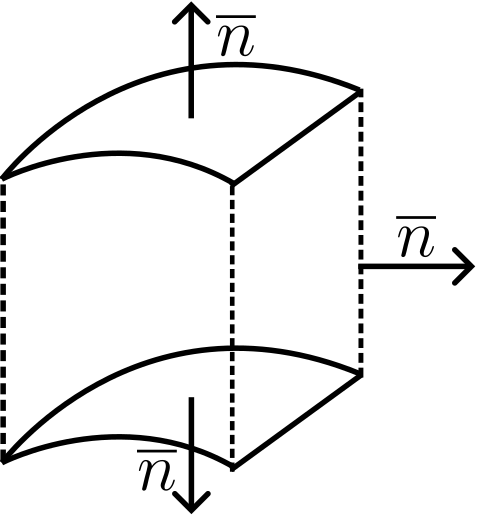
\includegraphics[scale=0.6]{8.22.1.png}
  \end{minipage}
  \hspace{1em}
  \begin{minipage}{0.55\textwidth}
    \[V=\iint_{D_{xy}}z_2(x;y)dxdy -\iint_{D_{xy}}z_1(x;y)dxdy=\]
    \[\iint_{S_2}z(x;y)dxdy+\iint_{S_1}z(x;y)dxdy+\iint_{S_3}\equalto{Z}{0}dxdy=\iint{\equalto{S}{S_1+S_2+S_3}}z dxdy\]
    S - внешняя сторона объемного тела
  \end{minipage}
  \vspace{1em}
  \par
  Аналогично можно получить: \[ V=\iint_S x dydz \hspace{20pt} V=\iint_S y dxdz\]
  Для поверхностей общего вида: \[V = \frac{1}{3}\iint_S xdydz+ydzdx+zdxdy=\frac{1}{3}\iint_S(x\cos(\alpha)+y\cos(\beta)+z\cos(\gamma))dS\]
  \subsection{Тройные интегралы}
  Пусть в некоторой пространственной области V задана функция $f(x;y;z)$
  \begin{enumerate}
    \item Произведем разбиение R
    \item В каждой элементарной области $V_i$ произвольно выберем (.) $\mu_i (\xi_i;\eta_i;\chi_i)$
    \item Вычислим $f(M_i)$
    \item Вычислим $f(M_i)\Delta V_i$
    \item Составим $\sigma_R=\sum_{i=1}^{n}f(M_i)\Delta V_i$
    \item Вычислим $\lim_{\lambda_R \to 0}\sigma_R=\iiint_V f(x;y;z)dv = \iiint_V f(x;y;z) dxdydz$
  \end{enumerate}
  \underline{Определение: } Если существует конечный предел интегральной суммы $\sigma_R$, не зависящий от выбора (.) $M_i$
  и способа разбиения пространственной области V, то она называется тройным интегралом от $f(x;y;z)$ по объемному телу V.\\
  Для существования интеграла $\Leftrightarrow \lim_{\lambda_R \to 0} (\overline{S}-\underline{S})=0$
  \[\begin{matrix}
    \underline{S}=\sum_{i=1}^{n}m_i V_i & m_i = \underset{(x_i;y_i;z_i) \in V_i}{inf f}\\
    \overline{S}=\sum_{i=1}^{n}m_i V_i & M_i = \underset{(x_i;y_i;z_i) \in V_i}{sup f}
  \end{matrix}\]
  Справедливы все свойства определенного интеграла.\\
  \break
  \underline{Вычисление тройного интеграла}\\
  \begin{minipage}{0.45\textwidth}
    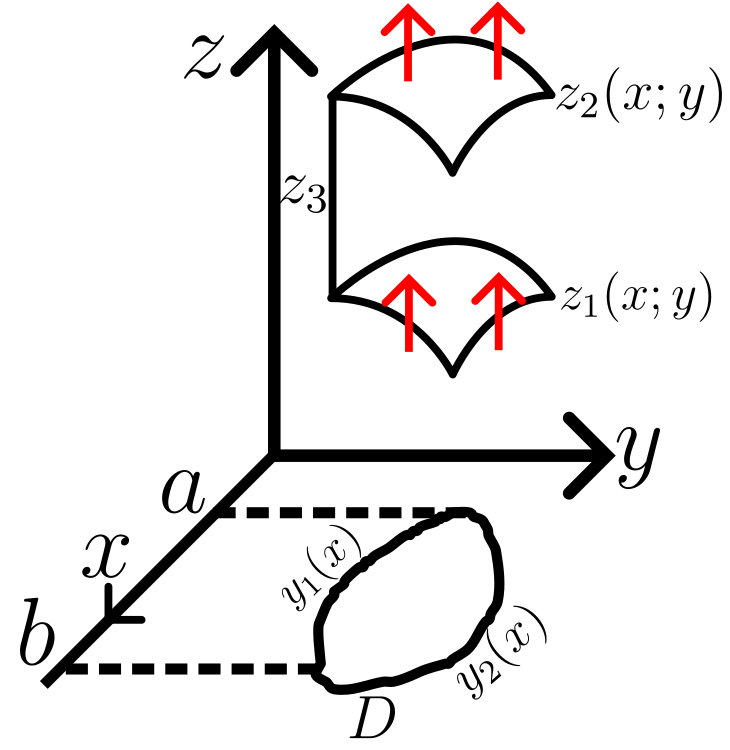
\includegraphics[scale=0.6]{8.23.1.png}
  \end{minipage}
  \hspace{1em}
  \begin{minipage}{0.55\textwidth}
    \[\iiint_V f(x;y;z) dxdydz = \iint_{D_{xy}}dxdy \Bigg[\int_{z_1(x;y)}^{z_2(x;y)}f(x;y;z)dz \Bigg]\]
    \[=\int_{a}^{b}dx \int_{y_1(x)}^{y_2(x)}\int_{z_1(x;y)}^{z_2(x;y)}dz=f(x;y;z)\]
  \end{minipage}
  \vspace{1em}
  \par
  \subsection{Формула Остроградского-Гаусса}
  Рассмотрим тело V, ограниченные кусочно-гладкими поверхностями. $\begin{matrix}
    S_1: z=z_1(x;y)\\
    S_2: z=z_2(x;y)\\
    S_3: \begin{matrix}
      \text{цилиндрическая поверхность}\\
      \text{с образующими || } OZ
    \end{matrix}
  \end{matrix}$\\
  Пусть в области V задана функция $R(x;y;z)$ непрерывная и имеет непрерывную частную производную $\frac{\delta R}{\delta z}$. 
  Тогда \[\iiint_V \frac{\delta R}{\delta z}dxdydz=\iint_S R dxdy\]
  \underline{Доказательство:}
    \[\text{Рассмотрим: }\underbrace{\iiint_V \frac{\delta R}{\delta z}dxdydz}=
    \iint_{D_{xy}}dxdy \Big[\int_{z_1(x;y)}^{z_2 (x;y)} \frac{\delta R}{\delta Z}dz\Big]=
    \iint_{D_{xy}}dxdy R(x;y;z_1(x;y))=\]
    \[\iint_{S_2}dxdy R(x;y;z)+
    \iint_{S_1}dxdy R(x;y;z)+
    \iint_{S_3}dxdy \equalto{R}{0}(x;y;z)=
    \underbracket{\iint_S dxdy R(x;y;z)}
    \]
  S - внешняя сторона поверхности, ограничивающей объемное тело V.
  \begin{center}
    \textbf{Ч.т.д.}
  \end{center}
  Аналогично: 
  \[\iiint_V \frac{\delta P}{\delta x}dxdydz = \iint_S P dydz \hspace{30pt} 
  \iiint_V \frac{\delta Q}{\delta y} dxdydz = \iint_S Q dxdz\]
  Общий вид:
  \[\iiint_V (\frac{\delta P}{\delta x}+\frac{\delta Q}{\delta y}+\frac{\delta R}{\delta z})dxdydz=
  \iint_S P dydz +Q dxdz+ R dxdy = 
  \iint_S(P\cos(\alpha)+Q\cos(\beta)+\cos(\gamma))dS\]
  \subsection{Замена переменных в тройном интеграле.}
  Рассмотрим две системы координат: $(x;y;z) \text{ и } (\xi,\eta,\chi)$\\
  Рассмотрим два замкнутых объемных тела: $V_D \in (x;y;z)$ \hspace{20pt} $V_D \in (\xi;\eta;\chi)$\\
  Оба тела ограничены поверхностями: $S \in (x;y;z) \hspace{20pt} \Sigma \in (\xi;\eta;\chi)$\\
  Пусть существует взаимно-однозначные соответствие между $(x;y;z)$ и $(\xi;\eta;\chi)$
  \[\begin{matrix}
    x=x(\xi;\eta;\chi)\\
    y=y(\xi;\eta;\chi)\\
    z=z(\xi;\eta;\chi)
  \end{matrix}\hspace{10pt}(1) \hspace{20pt}
  \begin{matrix}
    \xi=\xi(x;y;z)\\
    \eta=\eta(x;y;z)\\
    \chi=\chi(x;y;z)
  \end{matrix}\hspace{10pt}(2)\]
  \underline{Замечание:} при отображении (1) внутренней (.) переходит во внутреннюю, граничная (.) переходит в граничную.\\
  Пусть функции в (1)  имеют непрерывную частную производную.
  \[\text{Тогда} \hspace{10pt} \frac{D(x;y;z)}{D(\xi;\eta;\chi)} = I(\xi;\eta;\chi)=\begin{vmatrix}
    \frac{\delta x}{\delta \xi} & \frac{\delta x}{\delta \eta} & \frac{\delta x}{\delta \chi}\\
    \frac{\delta y}{\delta \xi} & \frac{\delta y}{\delta \eta} & \frac{\delta y}{\delta \chi}\\
    \frac{\delta z}{\delta \xi} & \frac{\delta z}{\delta \eta} & \frac{\delta z}{\delta \chi}\\
  \end{vmatrix}\]
  \[I(\xi;\eta;\chi)\not = 0 \text{ и сохраняет знак}\]
  Аналогично, как и в двойном интеграле, можно показать:
  \[\iiint_{V_D}dxdydz=\iiint_{V_\Delta}|I|d\xi d\eta d\chi\].
  \[|I|=\lim_{V_\Delta \to 0}\frac{V_D}{V_\Delta}\] Абсолютная величина Якобиана есть коэффициент растяжения(сжатия)
  пространства $(\xi;\eta;\chi)$ в пространство $(x;y;z)$\\
  \underline{Формула замены переменных в тройном интеграле:}
  \[\iiint_{V_D}f(x;y;z)dxdydz = \iiint_{V_\Delta}f(x(\xi;\eta;\chi);y(\xi;\eta;\chi);z(\xi;\eta;\chi))I d\xi d\eta d\chi\]
  \underline{Цилиндрическая система координат:}\\
  \begin{minipage}{0.45\textwidth}
    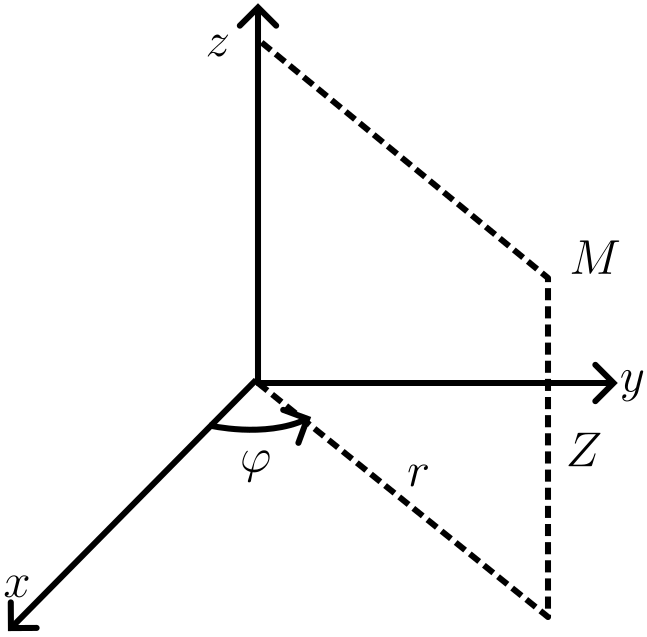
\includegraphics[scale=0.8]{8.25.1.png}
  \end{minipage}
  \hspace{1em}
  \begin{minipage}{0.55\textwidth}
    \[\begin{matrix}
      x=r\cos(\varphi)\\
      y=r\sin(\varphi)\\
      z=z
    \end{matrix}\hspace{20pt}
    I = \begin{vmatrix}
      -r\sin(\varphi) & \cos(\varphi) & 0\\
      r\cos(\varphi) & \sin(\varphi) & 0 \\
      0 & 0 & 1
    \end{vmatrix} =\]
    \[1 * A_{33}=M_{33}=-r\sin^2(\varphi)-r\cos^2(\varphi)=-r\]
    \[|I|=r\]
  \end{minipage}
  \vspace{1em}
  
  \par
  \underline{Сферическая система координат:}\\
  \par
  \begin{minipage}{0.45\textwidth}
    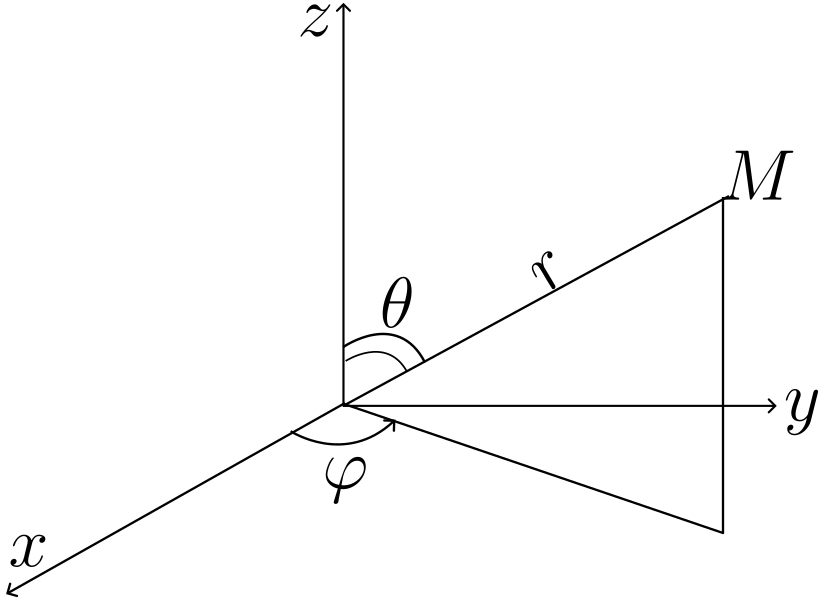
\includegraphics[scale=0.6]{8.25.2.png}
  \end{minipage}
  \hspace{1em}
  \begin{minipage}{0.55\textwidth}
    \[\varphi \in [0;2\pi]\]
    \[r \in [0;+\infty]\]
    \[\theta \in [0;\pi]\]
  \end{minipage}
  \vspace{1em}
  \par
  \begin{minipage}{0.45\textwidth}
    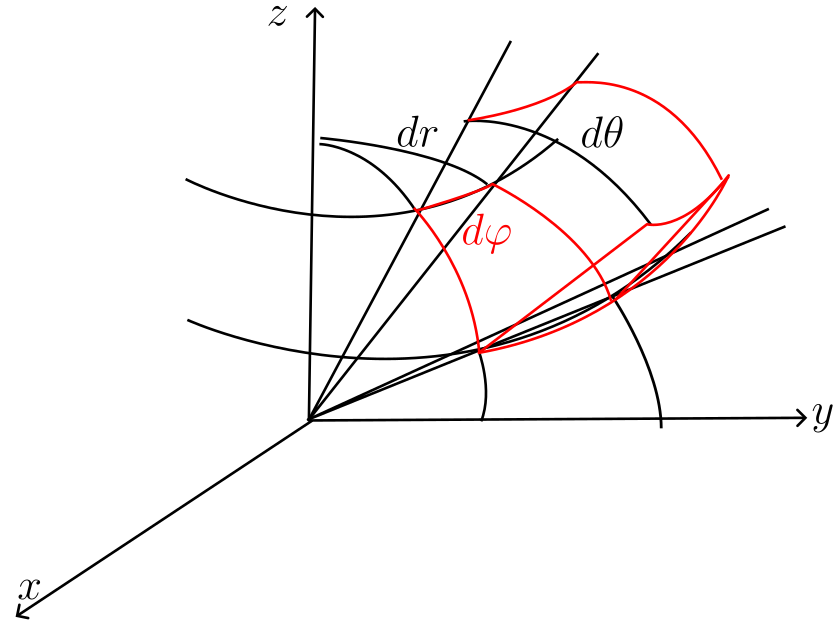
\includegraphics[scale=0.5]{8.25.3.png}
  \end{minipage}
  \hspace{1em}
  \begin{minipage}{0.55\textwidth}
    \[\begin{matrix}
      x=r\sin(\theta)\cos(\varphi)\\
      y=r\sin(\theta)\sin(\varphi)\\
      z=r\cos(\theta)
    \end{matrix}\]\[
    I = \begin{vmatrix}
      \sin(\theta)\cos(\varphi) & r\cos(\theta)\cos(\varphi) & -r\sin(\theta)\sin(\varphi)\\
      \sin(\theta)\sin(\varphi) & r\cos(\theta)\sin(\varphi) & -r\sin(\theta)\cos(\varphi)\\
      \cos(\theta)&-r\sin(\theta)&0
    \end{vmatrix}\]
    \[|I|=r^2\sin(\theta)\]
  \end{minipage}
  \vspace{1em}
  \par
  Рассмотрим сферу радиуса R с центром вращения в (.) (0;0;0)\\
  \begin{minipage}{0.45\textwidth}
    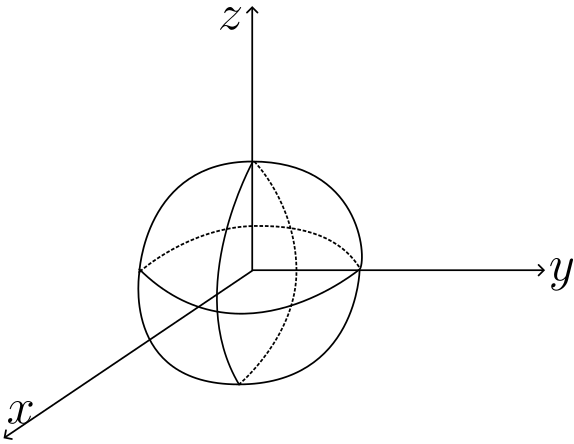
\includegraphics[scale=0.8]{8.25.4.png}
  \end{minipage}
  \hspace{1em}
  \begin{minipage}{0.55\textwidth}
    \[V-?\]
    \[V=\iiint_{V_D}dxdydz=\iiint_{V_\Delta}r^2\sin(\theta)drd\varphi d\theta=\]
    \[=\int_{0}^{2\pi}d\varphi \int_{0}^{\pi}d\theta \int_{0}^{R}dr r^2\sin(\theta)=
    \int_{0}^{2\pi}d\varphi \int_{0}^{\pi}d\theta \sin(\theta) \frac{R^3}{3}=\]
    \[=\frac{R^3}{3}\int_{0}^{2\pi}d\varphi 2=\frac{2}{3}R^3 2\pi=\frac{4 \pi R^3}{3}\]
  \end{minipage}
  \vspace{1em}
  \par
  \underline{Некоторые приложения тройного интеграла:}
  \begin{enumerate}
    \item \[V=\iiint_V dxdydz\]
    \item \[m=\iiint_V \rho(x;y;z)dxdydz\]
    \item \[
    \begin{matrix}
      M_{yz} = \iiint_{V} x\rho dxdydz & M_{xz}=\iint_V y \rho dxdydz & M_{xy}=\iint_V z\rho dxdydz\\
      x_c = \frac{M_{yz}}{m} & y_c=\frac{M_{xz}}{m} & z_c=\frac{M_{xy}}{m}
    \end{matrix}
    \]
  \end{enumerate}
  \subsection{n-кратные интегралы.}
  Рассмотрим $
  \begin{matrix}
    a_1 &\leq &x_1 &\leq &b_1\\
    a_2 &\leq &x_2 &\leq &b_2\\
    \vdots & &\vdots & & \vdots\\
    a_n &\leq &x_n &\leq &b_n
  \end{matrix}
  $
  \[P_n=[a_1 b_1][a_2 b_2]x\dots x[a_n b_n] \text{- n-мерный параллелепипед}\]
  Пусть в области V задана функция $y=f(x_1,\dots,x_n)$
  \begin{enumerate}
    \item Разбитие R объемного тела.
    \item Произвольным образов выберем (.) $\varepsilon_1,\dots,\varepsilon_n$.
    \item Вычислим $f(\varepsilon_1,\dots,\varepsilon_n)$
    \item Составим $\sigma_R=\sum_{i=1}^{n} f(\varepsilon_1,\dots,\varepsilon_n)\Delta V$
    \item $\lim_{\lambda_R \to 0} \sigma_R = \int \underset{V_n}{\dots} \int f(x_1,\dots,x_n)dx_1 \dots dx_n$
  \end{enumerate}
  \underline{Определение: } Если существует $\lim_{\lambda_R \to 0} \sigma_R$ независящей от R и выбора (.) $\varepsilon$,
  то он называется n-кратным интегралом от $f(x_1,\dots,x_n)$ по объемному телу V.\\
  \underline{Вычисление}\\
  Пусть V представима в виде: 
  \[\begin{matrix}
    x_1^* &\leq& x_1& \leq& x_1^1\\
    x_2^*(x_1) &\leq&x_2 &\leq&x_2^1(x_1)\\
    x_3^*(x_1;x_2)&\leq& x_3 &\leq&x_3^1(x_1;x_2)\\
                  &&\vdots&&\\
    x_n^*(x_1,\dots,x_{n-1})&\leq&x_n&\leq&x_n^1(x_1;\dots;x_{n-1})
  \end{matrix}\]
  \[\text{Тогда } \int \underset{V_n}{\dots} \int f(x_1;\dots;x_n) dx_1 \dots dx_n=
  \int_{x_1^*}^{x_1^1}dx_1 \int_{x_2^*(x_1)}^{x_2^1(x_1)}dx_2 \dots \int_{x_3^*(x_1;\dots;x_{n-1})}^{x_3^1(x_1;\dots;x_{n-1})}
  [f(x_1;\dots;x_n)]\]
  \underline{Замена переменных в n-кратном интеграле.}\\
  Пусть заданы 2 n-мерные области
  \[V_D \text{ и } V_\Delta\]
  \begin{minipage}{0.45\textwidth}
    \[\begin{cases}
      x_1&=x_1(\xi_1;\dots;\xi_n)\\
      \vdots&\\
      x_n&=x_n(\xi_1;\dots;\xi_n)
    \end{cases} \circled{1}\]
  \end{minipage}
  \hspace{1em}
  \begin{minipage}{0.55\textwidth}
    \[\begin{cases}
      \varepsilon_1&=\varepsilon_1(x_1;\dots;x_n)\\
      \vdots&\\
      \varepsilon_n&=\varepsilon_n(x_1;\dots;x_n)
    \end{cases} \circled{2}\]
  \end{minipage}
  \vspace{1em}
  \par
  \[\frac{D(x_1;\dots;x_n)}{D(\xi_1;\dots;\xi_n)}=I(\xi_1;\dots;\xi_n)
  \begin{vmatrix}
    \frac{\delta x_1}{\delta \xi_1}&\dots&\frac{\delta x_1}{\delta \xi_n}\\
    \vdots &&\vdots \\
    \frac{\delta x_n}{\delta \xi_1}&\dots&\frac{\delta x_n}{\delta \xi_n}
  \end{vmatrix}\]
  Пусть $I(\xi_1;\dots;\xi_n)\not =0$ и сохраняет знак в каждой (.).\\
  Тогда 
  \[\int \underset{V_D}{\dots} \int f(x_1;\dots;x_n)dx_1\dots dx_n = \int \underset{V_D}{\dots} \int 
  f(x_1(\xi_1;\dots;\xi_n);\dots;x_n(\xi_1;\dots;\xi_n)|I|d\xi_1\dots d\xi_n)\]
  \section{Теория Поля.}
  \subsection{Основные понятия.}
  \underline{Определения: }\\
  Скаляр - величина характеризующиеся своим числовым значением.\\
  Вектор - величина характеризующиеся числовым значением и направлением.\\
  Если с каждой (.) m некоторой пространственной области связана некоторая скалярная или векторная величина то говорят что
  задано поле этой величины. Заданное поле скалярной величины равносильно заданной скалярной функции и $(x;y;z)$.\\
  Чтобы задать векторное поле необходимо задать:
  \[A_x(x;y;z) \hspace{20pt} A_y(x;y;z) \hspace{20pt} A_z(x;y;z)\]
  \[\overline{A}=\underbracket{A_x i}_{P}+\underbracket{A_y j}_{Q}+\underbracket{A_z k}_{R}\]
  
  \begin{minipage}{0.55\textwidth}
    \underline{Определение: } Векторной линией называется кривая касательной которой в каждой ее (.) m совпадает
  с направление $\overline{A}$ отвечающим этой (.).\\
  \end{minipage}
  \hspace{1em}
  \begin{minipage}{0.45\textwidth}
    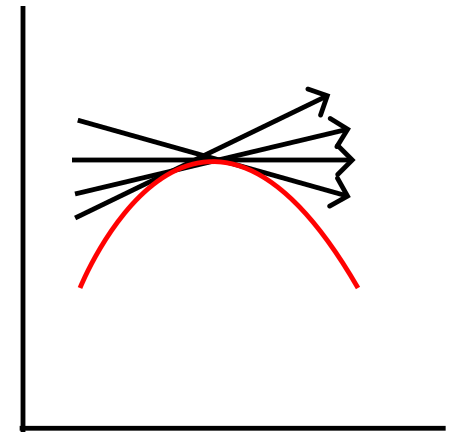
\includegraphics[scale=0.6]{9.1.png}
  \end{minipage}
  \vspace{1em}
  \par
  \underline{Определение: } Поверхность составленной из векторных линий называется векторной поверхностью.
  Характеризуется: в каждой ее (.) M. Соответствующий вектор $\overline{A}(M)$ лежит в касательной плоскости к
  этой поверхности в этой (.).
  Если взять в рассматриваемой области какую-нибудь линию отличную от векторной и через каждую ее
  (.) провести векторную линию то геометрическое место этих линий задает векторную поверхность.\\
  Если исходная линия была замкнутой, то полученная таким образом векторная поверхность называется 
  векторной трубкой.
  \break
  \subsection{Градиент}
  Пусть задана скалярное поле $u(x;y;z)$
  \[\overline{grad u} = \Big(\frac{\delta u}{\delta x};\frac{\delta u}{\delta y};\frac{\delta u}{\delta z}\Big)\]
  \[\frac{\delta u}{\delta l}=\overline{grad u} * \overline{l_0}=
  \frac{\delta u}{\delta x}\cos(\alpha)+
  \frac{\delta u}{\delta y}\cos(\beta)+
  \frac{\delta u}{\delta z}\cos(\gamma)\]
  \begin{center}
  Максимальное значение $\frac{\delta u}{\delta l}$ имеет в направлении вектора $\overline{gradu}$ 
  \end{center}
  \[\overline{\triangledown}\Big(\frac{\delta u}{\delta x};\frac{\delta u}{\delta y};\frac{\delta u}{\delta z}\Big)
  \overline{\triangledown} \text{- оператор Набла(оператор Гамильтона)}\]
  \[\overline{gradu}=\overline{\triangledown u}\]
  \subsection*{Дифференциальные свойства градиента}
  \begin{enumerate}
    \item \[\overline{grad}(u_1+u_2)=\overline{grad u_1}+\overline{grad u_2}\]
    \item \[\overline{grad(C_u)}=C\overline{grad u}, C=const\]
    \item \[\overline{grad}(u_1;u_2)=u_1\overline{grad u_2}+u_2\overline{grad u_1}\]
  \end{enumerate}
  \underline{Доказательство:}
  \begin{adjustwidth}{1.5em}{1.5em}
    \[\overline{grad}(u_1;u_2)=
    \frac{\delta}{\delta x}(u_1;u_2)\overline{i}+\frac{\delta}{\delta y}(u_1;u_2)\overline{j}+\frac{\delta}{\delta z}(u_1;u_2)\overline{k}=\]\[
    (u_1 \frac{\delta u_2}{\delta x}+u_2\frac{\delta u_1}{\delta x})\overline{i} + (u_1 \frac{\delta u_2}{\delta y}+u_2\frac{\delta u_1}{\delta y})\overline{j} + (u_1\frac{\delta u_2}{\delta z}+u_2\frac{\delta u_1}{\delta z})\overline{k}=\]
  
    \[u_1(\frac{\delta u_2}{\delta x}\overline{i} +\frac{\delta u_2}{\delta y}\overline{j}+\frac{\delta u_2}{\delta z}\overline{k})+
  u_2(\frac{\delta u_1}{\delta x}\overline{i} +\frac{\delta u_1}{\delta y}\overline{j}+\frac{\delta u_1}{\delta z}\overline{k})=\
  \]\[u_1 \overline{grad u_2}+u_2 \overline{grad u_1}\]
  \end{adjustwidth}
  \underline{Замечание:}Направление вектора градиента совпадает с направлением вектора нормали к поверхности уровня $u(x;y;z)=const.$\\
  \underline{Замечание:}Скалярное поле $u(x;y;z)$ порождает векторное поле градиента $\overline{grad u}(x;y;z)$

  \subsection{Поток вектора через поверхность.}
  Пусть задано векторное поле $\overline{A}(M)$, т.е. заданы функциями
  \[\begin{matrix}
    A_x(x;y;z)=P(x;y;z)\\
    A_y(x;y;z)=Q(x;y;z)\\
    A_z(x;y;z)=R(x;y;z)
  \end{matrix} \overline{A}(P;Q;R)\]
  Возьмем некоторую поверхность S, выбрав определенную ее строку\\
  \underline{Обозначение} $\overline{\cos(\alpha);\cos(\beta);\cos(\gamma)}=\overline{n_0}$\\
  \underline{Определение: } Потоком векторного поля $\overline{A}$ через поверхность S в сторону единичной нормали\\
  $\overline{n}(\cos(\alpha);\cos(\beta);\cos(\gamma))$ называется 
  \[\iint_S (P\cos(\alpha)+Q\cos(\beta))+\cos(\gamma)dS=\iint_S \overline{A} \overline{n}dS = \oiint_S A_n dS=\text{ П}\]
  Рассмотрим движение жидкости в пространстве. Движение нестационарное. Вычислим количество жидкости, протекающее
  через поверхность S в направлении $\overline{n}$ за малый промежуток времени $dt$. За время $dt$ через $ds$ протечет
  количество жидкости, которое заполняет собой цилиндр с основанием $ds$ и высотой $V_n dt$.\\
  \begin{minipage}{0.45\textwidth}
    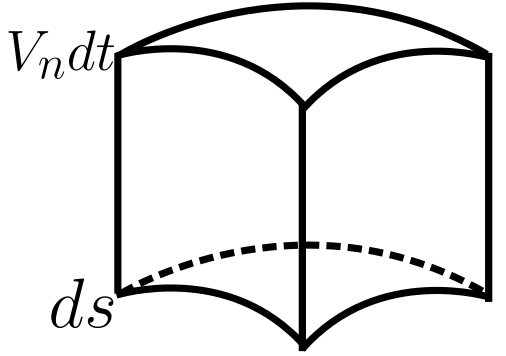
\includegraphics[scale=0.6]{9.2.png}
  \end{minipage}
  \hspace{1em}
  \begin{minipage}{0.55\textwidth}
    \[dm=\rho dV=\rho ds * V_n * dt\]
    \[m=dt \iint_{ds} V_n * \rho * ds\]
    \[\frac{m}{dt}=\iint_{ds} \rho V_n ds = Q\]
  \end{minipage}
  \vspace{1em}
  \par
  $Q$ - количество жидкости в единицу времени, поток вектора $\rho \overleftarrow{V_n}$ через поверхность S.\\
  Поток - скалярная величина, если угол между $\overline{A},\overline{n}$:
  \begin{itemize}
    \item острый $\Rightarrow$ П>0
    \item тупой $\Rightarrow$ П<0
    \item $\varphi = \frac{\pi}{2} \Rightarrow $ П=0
  \end{itemize}
  \[\text{П=} \iint_S (P\cos(\alpha)+Q\cos(\beta)+R\cos(\gamma))ds=\iiint_V
  (\frac{\delta P}{\delta x}+\frac{\delta Q}{\delta y}+\frac{\delta R}{\delta Z})dxdydz\]
  \underline{Определение: } Выражение 
  $\frac{\delta P}{\delta x}+\frac{\delta Q}{\delta y}+\frac{\delta R}{\delta Z}$ называется
  дивергенцией(расходимостью) векторного поля $\overline{A}$\\
  \underline{Обозначение:} $div \overline{A}$
  \[\text{П=} \iint_S \overline{A} \overline{n}dS=\iiint_V div \overline{A} dV\]
  \underline{Замечание:} Дивергенция - скаляр 
  \[\text{П=} \iiint_V div \overline{A} dV \underset{\hyperref[th:8.12.1]{\text{Th. о среднем}}}{=}
  \overline{A}\Big|_{(\xi,\eta,\chi)} \iiint_V dV= div\overline{A}\Big|_{(\xi,\eta,\chi)} *V \]
  \[div \overline{A} = \lim_{V \rightarrow (\xi,\eta,\chi)} \frac{\text{П}}{V}\]
  \subsection*{Физический смысл потока}
  Пусть $\overline{A}$ - векторное поле скоростей нестикаемой жидкости $(\rho = const)$ при наличии источников
  (стоков)
  \[\text{П} = \rho \iint_S \overline{V} \overline{n}dS\]
  \begin{itemize}
    \item П>0 - значит, что из области V, вытекает больше жидкости, чем втекает. Это означает, что внутри области
    V есть источники.
    \item П<0 - значит, что из области V вытекает меньше жидкости, чем втекает. Это означает что внутри области V есть стоки.
    \item П=0 - сколько жидкости втекает, столько и вытекает.
  \end{itemize}
  \subsection*{Физический смысл дивергенции:}
  Если источники(стоки) распределены непрерывно, то вводится понятие плотности источника(стока).
  \[div \overline{A}\Big|_M = \lim_{V \to M} \frac{\text{П}}{V} \text{- плотность источников(стоков)}\]
  \begin{itemize}
    \item $div \overline{A}\Big|_M >0$ - (.) M - источник.
    \item $div \overline{A}<0$ - (.) M - сток.
    \item $div\overline{A}\Big|_M = 0$ - (.) M ни источник, ни сток.
  \end{itemize}
  \subsection*{Свойства дивергенции:}
  \begin{enumerate}
    \item $div(\overline{a}+\overline{b})=div\overline{a}+div\overline{b}(\overline{a},\overline{b} - \text{векторные поля})$
    \item $div \overline{c} = 0, \overline{c} = const$
    \item $div(f\overline{a}) = f div\overline{a}+\overline{a}*\overline{gradf},$ f - скалярная функция $f(x,y,z)$
  \end{enumerate}
  \underline{Доказательство:}
  \begin{adjustwidth}{1.5em}{1.5em}
    \[div(f\overline{a})=\frac{\delta fP}{\delta X}+\frac{\delta f Q}{\delta y}+\frac{\delta f R}{\delta Z}=
    f\frac{\delta P}{\delta x}+P\frac{\delta f}{\delta x}+f \frac{\delta Q}{\delta y}+Q\frac{\delta f}{\delta y}+
    f\frac{\delta R}{\delta Z}+R\frac{\delta f}{\delta z}=\]
    \[f div \overline{a}+\overline{a}*\overline{gradf}\]
  \end{adjustwidth}
  \begin{center}
    \textbf{Ч.т.д.}
  \end{center}
  \underline{Замечание:} 
  \[\overline{\bigtriangledown} = \Big(\overline{\frac{\delta \underbracket{\hspace{10pt}}}{\delta x}
  ;\frac{\delta \underbracket{\hspace{10pt}}}{\delta y};\frac{\delta \underbracket{\hspace{10pt}}}{\delta z}}\Big)
  \text{ - оператор Гамильтона(оператор Набла)}\]
  \[div \overline{A} = \overline{\bigtriangledown}*\overline{A}\]
  \[\overline{\bigtriangledown} = \frac{\delta}{\delta x}\overline{i}+
  \frac{\delta}{\delta y}\overline{j}+\frac{\delta}{\delta z}\overline{k}\]

  \subsection{Циркуляция вектора}
  Пусть задано векторное поле $\overline{A}(P;Q;R)$ и замкнутая кривая $l$ в пределах рассматриваемой
  области.\\
  \underline{Определение: }$\int_{(l)} Pdx+Qdy+Rdz$ - называется \underline{циркуляцией} векторного поля
  $\overline{A}$ вдоль кривой l.\\
  \underline{Обозначение:} 
  \[\text{ц} = \oint_{(l)} Pdx+Qdy+Rdz= \oint_{(l)}[P\cos(\alpha)+Q\cos(\beta)+R\cos(\gamma)]dl=\]
  \[\oint_{(l)}(\overline{P;Q;R})(\overline{\cos(\alpha);\cos(\beta);\cos(\gamma)}dl=
  \oint_{(l)})\overline{A}*\overline{e}\]
  $\overline{e}$ - вектор, касательный к кривой в каждой(.)\\
  \underline{Замечание:} Если $\overline{A}$ - силовое поле, то Ц равна работе сил этого поля по
  перемещению (.) по кривой (l).
  \[\text{Ц=} \oint_{(l)} \overline{A}*\overline{e}dl \underset{\text{Формула Стокса}}{=}
  \iint_S \Big[\Big(\frac{\delta R}{\delta y}-\frac{\delta Q}{\delta z}\cos(\alpha)\Big)
  + \Big(\frac{\delta P}{\delta Z} - \frac{\delta R}{\delta x}\Big)\cos(\beta)
  + \Big(\frac{\delta Q}{\delta x}-\frac{\delta P}{\delta y}\cos(\gamma)\Big)\Big]dS\]
  \[\overline(n)(\cos(\alpha);\cos(\beta);\cos(\gamma)) - \text{нормаль к поверхности}\]
  \underline{Определение: } Вектор с координатами $\Big(\frac{\delta R}{\delta y}-\frac{\delta Q}{\delta z};
  \frac{\delta P}{\delta z}-\frac{\delta R}{\delta x};\frac{\delta Q}{\delta x} - \frac{\delta P}{\delta y}\Big)$
  называется ротором(вихрем) векторного поля $\overline{A}$.\\
  \underline{Обозначение: } $\overline{rotA}$
  \[\oint_{(l)}\overline{A}\overline{e}dl = \iint_S \overline{rotA}*\overline{n_0}dS = \text{ц}\]
  То есть циркуляция векторного поля $\overline{A}$ вдоль замкнутого контура l равна потоку ротора этого поля
  $\overline{rotA}$ через поверхность S, границей которого является l.
  \[\overline{rotA} = \overline{\bigtriangledown} X \overline{A} = 
  \begin{vmatrix}
    \overline{i} & \overline{j} &\overline{k}\\
    \frac{\delta}{\delta x} & \frac{\delta }{\delta y} & \frac{\delta }{\delta z}\\
    P & Q & R
  \end{vmatrix}\]
  \subsection*{Свойство ротора:}
  \begin{enumerate}
    \item $\overline{rot}(\overline{a}+\overline{b}) = \overline{rota}+\overline{rotb}$
    \item $\overline{rot}(f\overline{a}) = f\overline{rota}+\overline{gradf}X\overline{a}$
  \end{enumerate}
  \pagebreak
  \underline{Доказательство:}
  \begin{adjustwidth}{1.5em}{1.5em}
    \[\overline{rot}(f\overline{a}) = 
    \begin{vmatrix}
      \overline{i} & \overline{j} &\overline{k}\\
      \frac{\delta}{\delta x} & \frac{\delta }{\delta y} & \frac{\delta }{\delta z}\\
      fP & fQ & fR
    \end{vmatrix} = 
    i\Big(\frac{\delta fR}{\delta y} - \frac{\delta f Q}{\delta z}\Big) 
   -j\Big(\frac{\delta fR}{\delta x} - \frac{\delta f P}{\delta z}\Big)
   +k\Big(\frac{\delta fQ}{\delta x} - \frac{\delta f P}{\delta y}\Big)=\]
    \[=i\Big(\frac{\delta f}{\delta y}R + f\frac{\delta R}{\delta y} - \frac{\delta f}{\delta z}Q-f\frac{\delta Q}{\delta z}\Big)-
    j\Big(\frac{\delta f}{\delta x}R + \frac{\delta R}{\delta x}f - \frac{\delta f}{\delta z}P - f\frac{\delta P}{\delta z}\Big)+
    k\Big(\frac{\delta f}{\delta x}Q+\frac{\delta Q}{\delta x}P - \frac{\delta f}{\delta y}P - f\frac{\delta P}{\delta y}\Big)=\]
    \[f\Big(\frac{\delta R}{\delta y}-\frac{\delta Q}{\delta z};
        \frac{\delta P}{\delta z}-\frac{\delta R}{\delta x};
        \frac{\delta Q}{\delta x}-\frac{\delta P}{\delta y}\Big)=
    \begin{vmatrix}
      \overline{i} & \overline{j} &\overline{k}\\
      \frac{\delta}{\delta x} & \frac{\delta }{\delta y} & \frac{\delta }{\delta z}\\
      P & Q & R
    \end{vmatrix}=\]
    \[f * \overline{rot}\overline{a}+\overline{grad}f x \overline{a}\]
  \end{adjustwidth}
  \begin{enumerate}
    \setcounter{enumi}{2}
    \item Если $\overline{c}=const,\overline{rot} \overline{c}=\overline{0}$
    \item Если $\overline{r}=x \overline{i}+y\overline{j}+z\overline{k},\overline{rot}\overline{r} = \overline{0}$
  \end{enumerate}
  \subsection*{Формула Стокса:}
  \[\int_{(l)} = \overline{A}\overline{e}dl 
  = \iint_S \overline{rot}\overline{A}*\overline{n_0} dS 
  = \iint_S rot A_n dS
  = rot A_n \Big|_{(\xi,\eta,\chi)} \iint_S dS\]
  \[rot A_n = \lim_{(S) \to M} \frac{\int_{(l)} \overline{A}\overline{e}dl}{S}\]
  Ротор - это вектор, проекция которого на каждое направление равна пределу отношения циркуляции векторного
  поля по кривой l плоской площади, перпендикулярной к этому направлению, к площади этой площади, 
  когда площадка стягивается в точку.\\
  \underline{Замечание:} Если $\overline{A}$ - векторное поле скоростей, то 
  $\overline{rot}\overline{A} = \overline{\omega}$ - угловая скорость.
  \subsection*{Дифференциальные операции второго порядка:}
  \begin{enumerate}
    \item $div \overline{grad}u= \overline{\bigtriangledown}(\overline{\bigtriangledown} u) = 
    \frac{\delta }{\delta x}*\frac{\delta u}{\delta x}+
    \frac{\delta}{\delta y}*\frac{\delta  u}{\delta y}+
    \frac{\delta}{\delta z}*\frac{\delta u}{\delta z}=
    \frac{\delta^2 u}{\delta x^2}+\frac{\delta^2 u}{\delta y^2}+\frac{\delta^2 u}{\delta z^2}$
    \[\text{Оператор }\bigtriangleup = 
    \frac{\delta^2}{\delta x^2 }+\frac{\delta^2}{\delta y^2}+\frac{\delta^2}{\delta z^2} \text{ - оператор Лапласа}\]
    \[div\overline{grad}u=\bigtriangleup u\]

    \item $\overline{rot} \overline{gradu} = 
    \begin{vmatrix}
      i & j & k\\
      \frac{\delta}{\delta x} & \frac{\delta}{\delta y} & \frac{\delta}{\delta z}\\
      \frac{\delta u}{\delta x} & \frac{\delta u}{\delta y} & \frac{\delta u}{\delta z}
    \end{vmatrix}
    =i\Big(\frac{\delta^2 u}{\delta y \delta z}-\frac{\delta^2 u}{\delta y \delta z}\Big)
    -j\Big(\frac{\delta^2 u}{\delta x \delta z}-\frac{\delta^2 u}{\delta x \delta z}\Big)
    +k\Big(\frac{\delta^2 u}{\delta x \delta y}-\frac{\delta^2 u}{\delta x \delta y}\Big)=
    \overline{o}$

    \item $\overline{grad}div \overline{A}=\overline{\bigtriangledown}(\bigtriangledown A)=
    \frac{\delta}{\delta x}\Big(\frac{\delta P}{\delta x}+\frac{\delta Q}{\delta y}+\frac{\delta R}{\delta z}\Big)\overline{i}
  + \frac{\delta}{\delta y}\Big(\frac{\delta P}{\delta x}+\frac{\delta Q}{\delta y}+\frac{\delta R}{\delta z}\Big)\overline{j}
  + \frac{\delta}{\delta z}\Big(\frac{\delta P}{\delta x}+\frac{\delta Q}{\delta y}+\frac{\delta R}{\delta z}\Big)\overline{k}
  = \overline{i}\Big(\frac{\delta^2 P}{\delta x^2}+\frac{\delta^2 Q}{\delta x \delta y}+\frac{\delta^2 R}{\delta x \delta z}\Big)
  + \overline{j}\Big(\frac{\delta^2 P}{\delta x \delta y}+\frac{\delta^2 Q}{\delta y^2}+\frac{\delta^2 R}{\delta x \delta z}\Big)
  + \overline{k}\Big(\frac{\delta^2 P}{\delta x \delta y}+\frac{\delta^2 Q}{\delta y \delta z}+\frac{\delta^2 R}{\delta z^2}\Big)$
    
    \item $div \overline{rot}\overline{A} = \frac{\delta}{\delta x}\Big(\frac{\delta R}{\delta y}-\frac{\delta Q}{\delta z}\Big)
    + \frac{\delta}{\delta y}\Big(\frac{\delta P}{\delta z} - \frac{\delta R}{\delta x}\Big)+
    \frac{\delta}{\delta z }\Big(\frac{\delta Q}{\delta x} - \frac{\delta P}{\delta y}\Big)=0$

    \item $\overline{rot}\overline{rotA} =
    \begin{vmatrix}
      \overline{i} & \overline{j} & \overline{k}\\
      \frac{\delta}{\delta x} & \frac{\delta}{\delta y} & \frac{\delta}{\delta z}\\
      \frac{\delta R}{\delta y} - \frac{\delta Q}{\delta z} & 
      \frac{\delta P}{\delta z} - \frac{\delta R}{\delta x} &
      \frac{\delta Q}{\delta x} - \frac{\delta P}{\delta y}
    \end{vmatrix}
    =\overline{i}\Big(\frac{\delta^2 Q}{\delta x \delta y} - \frac{\delta^2 R}{\delta y^2}-
    \frac{\delta^2 P}{\delta z^2} + \frac{\delta^2 R}{\delta x \delta z}-\frac{\delta^2 P}{\delta x^2}+\frac{\delta^2 P}{\delta x^2}\Big)-
    \overline{j}\Big(\frac{\delta^2 Q}{\delta x^2} - \frac{\delta^2 P}{\delta x \delta y} - \frac{\delta^2 R}{\delta y \delta z} +
    \frac{\delta^2 Q}{\delta z^2}+\frac{\delta^2 Q}{\delta y^2}-\frac{\delta^2 Q}{\delta y^2}\Big)+
    \overline{k}\Big(\frac{\delta^2 P}{\delta x \delta z} - \frac{\delta^2 R}{\delta x^2} - \frac{\delta^2 R}{\delta y^2}+
    \frac{\delta^2 Q}{\delta y \delta z} - \frac{\delta^2 R}{\delta z^2}+ \frac{\delta^2 R}{\delta z^2}\Big)=
    \overline{i}\Big(\frac{\delta^2 P}{\delta x^2}+\frac{\delta^2 Q}{\delta x \delta y}+\frac{\delta^2 R}{\delta x \delta z}\Big)+
    \overline{j}\Big(\frac{\delta^2 Q}{\delta y^2}+\frac{\delta^2 P}{\delta x \delta y}+ \frac{\delta^2 R}{\delta y \delta z}\Big)+
    \overline{k}\Big(\frac{\delta^2 R}{\delta z^2}+\frac{\delta^2 P}{\delta x \delta z} + \frac{\delta^2 Q}{\delta y \delta z}\Big)-
    \overline{i}\Big(\frac{\delta^2 P}{\delta x^2}+\frac{\delta^2 P}{\delta y^2}+\frac{\delta^2 P}{\delta z^2}\Big)-
    \overline{j}\Big(\frac{\delta^2 Q}{\delta x^2}+\frac{\delta^2 Q}{\delta y^2}+\frac{\delta^2 Q}{\delta z^2}\Big)-
    \overline{j}\Big(\frac{\delta^2 R }{\delta x^2}+\frac{\delta^2 R}{\delta y^2}+\frac{\delta^2 R}{\delta z^2}\Big)=
    \overline{grad}div \overline{A}=\overline{\bigtriangleup A}$
    \[\overline{\bigtriangleup A}(\Delta P;\Delta Q;\Delta R)\]
\end{enumerate}
\subsection{Виды векторных полей}
\begin{enumerate}
  \item Потенциальное поле\\
  \underline{Определение: } Векторное поле $\overline{A}$ называется потенциальным, если существует скалярная функция,
  для которой $\overline{A}$ является градиентом.
  \[\overline{A}=\overline{gradu},\text{т. е.}\]
  \[P=\frac{\delta u}{\delta x};Q=\frac{\delta u}{\delta y}; R= \frac{\delta u}{\delta z}\]
  \[Pdx+Qdy+Rdz=du\]
  \underline{Определение: } Функция $u(x;y;z)$ называется потенциальной функцией поля $\overline{A}$.\\
  \underline{Утверждение: } Для того чтобы поле $\overline{A}$ было потенциальным $\Leftrightarrow$ чтобы 
  \[\frac{\delta R}{\delta y}=\frac{\delta Q}{\delta z};\frac{\delta P}{\delta z}=\frac{\delta R}{\delta x};
  \frac{\delta Q}{\delta x}=\frac{\delta P}{\delta y} \Rightarrow \boxed{\overline{rot}\overline{A}=\overline{o}}\]
  Потенциальное поля называют безвихревым полем.\\
  Для потенциального поля справедливо:
  \begin{itemize}
    \item Циркуляция по простому замкнутому контуру всегда равна 0.
    \item Интеграл по кривой, соединяющий две (.) поля, не зависит от формы кривой(не зависит от пути интегрирования).
    \item  Скалярная функция u определяется с точностью до постоянной.
  \end{itemize}
  \item Соленоидальное поле\\
  \underline{Определение: } Векторное поле А называется соленоидальным(трубчатым), если существует
  функция $\overline{B}$, для которой А служит ротором.
  \[\overline{A}=\overline{rot}\overline{B}; 
  A_x=\frac{\delta B_z}{\delta y}-\frac{\delta B_y}{\delta z};
  A_y=\frac{\delta B_x}{\delta z}-\frac{\delta B_z}{\delta x};
  A_z=\frac{\delta B_y}{\delta x}-\frac{\delta B_x}{\delta y}\]
  $\overline{B}$ называется векторным потенциалом поля $\overline{A}$.\\
  \underline{Утверждение: } Для того чтобы векторное поле было соленоидальным $\Leftrightarrow \boxed{\overline{div}\overline{A}=0}$\\
  \pagebreak
  \underline{Доказательство:}
  \begin{adjustwidth}{1.5em}{1.5em}
    \circled{$\Rightarrow$} Поле соленоидальное, тогда по определению существует $\overline{B}:A=\overline{rot}\overline{B}$. 
    Вычислим $div\overline{A}=div(\overline{rot}\overline{B})=0$\\
    \circled{$\Leftarrow$} Пусть $div \overline{A}=0.$ Надо показать, что существует $\overline{B}:A=\overline{rot}\overline{B}$
    \[(\overline(A_x;A_y;A_z)) \text{ - известно} \hspace{20pt} 
    (\overline{B_x;B_y;B_z}) \text{ - неизвестно}\]
    Достаточно найти какое-нибудь одно частное решение.
    Пусть $B_z=0$
    \[A_x = - \frac{\delta B_y}{\delta B_z}; \hspace{10pt}
      A_y = \frac{\delta B_x}{\delta B_z}; \hspace{20pt}
      A_z = \frac{\delta B_y}{\delta x} - \frac{\delta B_x}{\delta y}\]
    \[B_y = - \int_{z_0}^{z}A_x(x;y;z)dz+p(x;y) ; \hspace{20pt}
      B_x = \int_{z_0}^{z}A_y(x;y;z)dz\]
      Найдем $\varphi(x;y)$
      \[\frac{\delta B_y}{\delta x}= - \int_{z_0}^{z}\frac{\delta A_x}{\delta x}dz+\varphi'_x(x;y) \hspace{20pt}
      \frac{\delta B_x}{\delta y} = \int_{z_0}^{z}\frac{\delta A_y}{\delta y}dz\]
      Тогда
      \[A_z = - \int_{z_0}^{z}\Big[\frac{\delta A_x}{\delta x}+ \frac{\delta A_y}{\delta y}\Big]dz
      +\varphi'_x(x;y)=
      \begin{vmatrix}
        \frac{\delta A_x}{\delta x}+\frac{\delta A_y}{\delta y}+\frac{\delta A_z}{\delta z}=0\\
        \frac{\delta A_x}{\delta x }+\frac{\delta A_y}{\delta y}= -\frac{\delta A_z}{\delta z}
      \end{vmatrix}=\]
      \[=\int_{z_0}^{z}\frac{\delta A_z}{\delta z}dz + \varphi'_x(x;y)=A_z(x;y;z)-A_z(x;y;z_0)+\varphi'_x(x;y) \Rightarrow\]
      \[\varphi'_x(x;y)=A_z(x;y;z_0) \hspace{20pt} \varphi(x;y)=\int_{x_0}^{x}A_z(x;y;z_0)dx+\psi(y)\]
      \[B_x=\int_{z_0}^{z}A_y(x;y;z)dz \hspace{20pt} 
      B_y = - \int_{z_0}^{z}A_x(x;y;z)dz+\int_{x_0}^{x}A_z(x;y;z_0)dx+\psi(y) \hspace{20pt}
      B_z =0\]
    \end{adjustwidth}
    \begin{center}
      \textbf{Ч.т.д.}
    \end{center}
    \item Разложение произвольного векторного поля.\label{punkt3} \\
    Пусть A - произвольное векторное поле.
    \begin{itemize}
      \item $\overline{A}=\overline{A}'+\overline{A}''$
      \item $\overline{A}'$ - потенциальная составляющая($\overline{rot}\overline{A}=0$)
      \item $\overline{A}''$ - соленоидальная составляющая ($div \overline{A}'=0$)
    \end{itemize}
    Пусть $F$ - скалярная функция. \hspace{20pt} $F-?$ \hspace{10pt} Пусть $\overline{A}' = \overline{gradF} \hspace{20pt} rotgradF=0$\\
    Тогда $\overline{A}'' = \overline{A}-\overline{A}'$.
    \[div \overline{A}'' = div\overline{A}' = div \overline{A}-divgradF=div \overline{A}-\Delta F=0 \hspace{10pt} \Delta F=divA\]
    \clearpage
    \underline{Алгоритм:}
    \begin{enumerate}
      \item[1.] $\Delta F = divA \Rightarrow F$
      \item[2.] $\overline{A}' = gradF$
      \item[3.] $\overline{A}'' = \overline{A} - \overline{A}'$
    \end{enumerate}
    \item Гармоническое поле\\
    \underline{Определение: } Векторное поле $\overline{A}$ называется гармоническим, если оно и потенциальное и
    соленоидальное одновременное; т.е.
    \[div \overline{A} = 0 \hspace{20pt} \overline{rot}\overline{A}=0\]
    Пусть $F$ - скалярная функция \hspace{20pt} $F-?$\\
    Пусть $\overline{A} = \overline{grad}F(\overline{rot}\overline{A}=rot\overline{grad}F=0)$
    \[div \overline{A} = div\overline{grad}F=0 \hspace{20pt} \Delta F=0\]
    Алгоритм
    \[\frac{\delta^2 F}{\delta x^2}+\frac{\delta^2 F}{\delta y^2}+\frac{\delta^2 F}{\delta z^2} = 0 \Rightarrow F\]
    \[\overline{A}=\overline{grad}F\]
    \item Обратная задача векторного анализа\\
    \underline{Задача}: Найти векторное поле $A$, если известно
    \[div \overline{A} = F \hspace{20pt} \overline{rot}\overline{A}=\overline{B}\]
    \underline{Решение}
    \begin{center}
      Решение ищем в виде: $\overline{A}=\overline{A'}+\overline{A''}$
    \end{center}
    \[(1):\begin{matrix}
      \overline{rot}\overline{A'}=0\\
      div \overline{A'}=F
    \end{matrix}
    \hspace{20pt} 
    (2):\begin{matrix}
      \overline{rot} \overline{A''}=\overline{B}\\
      div \; A'' = 0
    \end{matrix}\]
    \begin{enumerate}
      \item[(1):] Пусть Ф - скалярная функция. Тогда $\overline{A'}$ можно представить в виде
      \[\overline{A'}=\overline{\text{gradФ}},\text{т.к. } \overline{rot}\overline{grad}\text{Ф}=0\]
      Тогда $div \overline{A'}=div\overline{grad}\text{Ф}=\Delta \text{Ф}=F$\\
      \underline{Алгоритм:}
      \begin{enumerate}
        \item[1.] $\Delta \text{Ф}=F \hspace{20pt} \text{Находим Ф}$
        \item[2.] $\overline{A'}=\overline{grad}\text{Ф}$ 
      \end{enumerate}
      \item[(2):] $\overline{rot}\overline{A''}=\overline{B}$\\
      $\overline{B}$ известно. Тогда из \hyperref[punkt3]{пункта 3} можно найти частное решение
      $\overline{A_0''}$. Общее решение ищем в виде:
      \[\overline{A''}=\overline{A_0''}+\overline{C},\text{где } 
      \overline{C}=\overline{grad\tilde{\text{Ф}}}(\text{нужно, чтобы }
      \overline{rot}\overline{C}=0)\]
      \underline{Алгоритм:}
      \begin{enumerate}
        \item[1)] Решаем уравнение $\overline{rot}\overline{A''}=B$
        \item[2)] Решаем $\Delta \tilde{\text{Ф}}=-div\overline{A_0''}$. Находим $\tilde{\text{Ф}}$
        \item[3)] Находим $\overline{C}=grad \tilde{\text{Ф}}$
        \item[4)] $\overline{A''}=\overline{A_0''}+\overline{C}$
      \end{enumerate}
    \end{enumerate}
  \end{enumerate}
  %КОНЕЦ 3 СЕМЕСТРА ЛЮБИМОГО МАТ АНАЛИЗА ААААААААААААААААААААААА
\end{document}